\documentclass{report}
\usepackage{tikz}
\usepackage{amsmath}
\usepackage{amsthm}
\usepackage{amssymb}
\usepackage{bbold}
\usepackage{graphicx}
\usepackage{geometry}
\usepackage{nicematrix}
\usepackage{natbib}
\usepackage[hidelinks]{hyperref}
\usepackage{subcaption}

\geometry{
  paper=a4paper,
  margin=59pt,
  includeheadfoot
}

\graphicspath{{images/}}

\bibliographystyle{dinat}

\theoremstyle{definition}
\newtheorem{theorem}{Theorem}[chapter]
\newtheorem{corollary}[theorem]{Corollary}
\newtheorem{lemma}[theorem]{Lemma}
\newtheorem{observation}[theorem]{Observation}
\newtheorem{problem}[theorem]{Problem}
\newtheorem{definition}{Definition}[chapter]
\newtheorem{algorithm}{Algorithm}[chapter]
\newtheorem{example}[definition]{Example}

\newcommand{\R}{\mathbb{R}}
\newcommand{\N}{\mathbb{N}}
\newcommand{\Z}{\mathbb{Z}}
\newcommand{\Q}{\mathbb{Q}}
\newcommand{\T}{\mathbb{T}}
\renewcommand{\d}{\,\mathrm{d}}
\newcommand{\imat}{\mathbb{1}}
\newcommand{\zeromat}{\mathbb{0}}
\newcommand{\sprod}[2]{\langle #1 \mid #2 \rangle}
\newcommand{\largesprod}[2]{\left\langle #1 \,\middle|\, #2 \right\rangle}
\newcommand{\powerset}{\mathcal{P}}
\newcommand{\lagrangian}{\mathcal{L}}
\DeclareMathOperator{\opvec}{vec}
\DeclareMathOperator{\opmat}{mat}
\DeclareMathOperator{\solspace}{Sol}
\DeclareMathOperator{\GL}{GL}
\DeclareMathOperator{\rank}{rank}
\DeclareMathOperator{\nullity}{nullity}
\DeclareMathOperator{\Span}{span}
\DeclareMathOperator{\im}{im}
\DeclareMathOperator{\aff}{aff}
\DeclareMathOperator{\conv}{conv}

\setcounter{secnumdepth}{3}
\setcounter{tocdepth}{3}

\newcommand{\mat}[1]{\left(\begin{matrix}#1\end{matrix}\right)}
\newcommand{\smat}[1]{\left(\begin{smallmatrix}#1\end{smallmatrix}\right)}

\newcommand\restrict[2]{{% we make the whole thing an ordinary symbol
  \left.\kern-\nulldelimiterspace % automatically resize the bar with \right
  #1 % the function
  \vphantom{\big|} % pretend it's a little taller at normal size
  \right|_{#2} % this is the delimiter
  }}


\begin{document}

\begin{titlepage}
  \centering
  \vspace*{0.5cm}
  
\includegraphics[width=0.4\textwidth]{uni_jena_logo.png}\par
  \vspace{1cm}
  {\LARGE\textbf{Reducing Integer Linear Programs to Shortest Path Problems}\par}
  \vspace{1.5cm}
  {\Large \textsc{Bachelor Thesis}\par}
  \vspace{1.5cm}
  {\Large To obtain the academic degree\par}
  \vspace{0.5cm}
  {\Large Bachelor of Science (B.Sc.) in Applied Computer Science\par}
  \vspace{1.5cm}
  {\Large \textsc{Friedrich-Schiller-Universität Jena}\par}
  \vspace{0.5cm}
  {\Large Fakultät für Mathematik und Informatik\par}
  \vspace{0.5cm}
  {\Large \par}
  \vfill
  {\large Moritz Seppelt\par}
  {\large Born Janurary 27, 2001 in Braunschweig, Germany\par}
  \vspace{0.5cm}
  {\large Supervisor: Joachim Giesen, Univ.-Prof. Dr \par}
  \vfill
  {\large Jena, Germany\par}
  {\large March 7, 2024\par} % Replace with submission date
\end{titlepage}

\newpage
\thispagestyle{empty}
\begin{center}
    \Large\textbf{Abstract}
\end{center}

Integer linear programming (ILP) serves as a foundational framework for solving optimization problems with discrete decision variables, finding applications across diverse domains like operations research, logistics, finance, and bioinformatics. In \textit{Algebraic statistics for computational biology} by Lior Patcher and Bernd Sturmfels, a method was introduced, demonstrating the resolution of specific ILP instances by transforming them into shortest path problems on directed, weighted graphs. However, the original approach was limited to ILPs where the columns of the constraint matrix sum to the same value. This thesis revisits and extends this methodology to accommodate a broader class of ILP instances. Specifically, we consider ILPs of the form $A\vec x = \vec b$, where $A\in \mathbb{Z}^{m \times n}$, $\vec x \in \mathbb{N}^n$, and $\vec b \in \mathbb{Z}^m$. Unlike prior work, we relax the constraint on the column sums of $A$, allowing for variability provided they remain strictly positive. To achieve this, I translate the ILP into a form amenable to the proposed algorithm, involving the conversion of constraints into a graph representation suitable for shortest path computation. This translation introduces a crucial degree of freedom, influencing algorithm performance. The thesis aims to explore and exploit this flexibility to enhance the algorithm's  efficiency for ILPs with varying column sums. Through this work, I aim to contribute to the understanding ILPs.
\vspace{1.5cm}
\begin{center}
  \Large\textbf{Zusammenfassung}
\end{center}

Ganzzahlige lineare Programmierung (ILP) dient als grundlegender Rahmen für die Lösung von Opti-mierungsproblemen mit diskreten Entscheidungsvariablen und findet in verschiedenen Bereichen wie Operations Research, Logistik, Finanzen und Bioinformatik Anwendung. In \textit{Algebraic statistics for computational biology} von Lior Patcher und Bernd Sturmfels wurde eine Methode vorgestellt, die die Lösung spezifischer ILP-Instanzen durch Umwandlung in kürzeste Wege Problemen auf gerichteten, gewichteten Graphen demonstriert. Der ursprüngliche Ansatz war jedoch auf ILPs beschränkt, bei denen die Summe der Spalten der Constraint-Matrix denselben Wert ergibt. In dieser Arbeit wird diese Methodik überarbeitet und erweitert, um eine breitere Klasse von ILP-Instanzen zu berücksichtigen. Konkret betrachten wir ILPs der Form $A\vec x = \vec b$, wobei $A\in \mathbb{Z}^{m \times n}$, $\vec x \in \mathbb{N}^n$ und $\vec b \in \mathbb{Z}^m$. Im Gegensatz zu früheren Arbeiten lockern wir die Beschränkung auf die Spaltensummen von $A$ und lassen Variabilität zu, sofern sie positiv bleiben. Um dies zu erreichen, übersetze ich das ILP in eine Form, die für den vorgeschlagenen Algorithmus geeignet ist, indem ich die Nebenbedingungen in eine Graphendarstellung umwandle, die für die Berechnung des kürzesten Weges geeignet ist. Diese Übersetzung führt einen entscheidenden Freiheitsgrad ein, der die Leistung des Algorithmus beeinflusst. Ziel dieser Arbeit ist es, diese Flexibilität zu erforschen und auszunutzen, um die Effizienz des Algorithmus für ILPs mit variierenden Spaltensummen zu verbessern. Mit dieser Arbeit möchte ich einen Beitrag zum Verständnis von ILPs leisten.



\tableofcontents

\chapter{Framework}
\section{Introduction}
\section{Graphs}
\begin{figure}[ht]
    \centering
    \begin{tikzpicture}[->,shorten >=1pt,auto,node distance=3cm,semithick]

    
      \node[circle, draw, fill=white, inner sep=2pt] (v1) {$v_1$};
      \node (v2) [below of=v1] {$v_2$};
      \node (v3) [right of=v2] {$v_3$};
      \node (v5) [right of=v1] {$v_5$};
      \node (v4) [right of=v5, below of=v5] {$v_4$};
    
      \path (v1) edge node {3} (v2)
            (v2) edge node {5} (v3)
            (v3) edge node {2} (v4)
            (v4) edge node {4} (v5)
            (v5) edge node {1} (v1)
            (v1) edge [loop left] node {6} (v1)
            (v3) edge node {7} (v5);
    \end{tikzpicture}
    \caption{Weighted Directed Graph with 5 Nodes}
\end{figure}

\begin{align*}
    A = \begin{bmatrix}
    \infty & 3 & \infty & \infty & \infty \\
    \infty & \infty & 5 & \infty & \infty \\
    \infty & \infty & \infty & 2 & 7 \\
    \infty & \infty & \infty & \infty & 4 \\
    1 & \infty & \infty & \infty & \infty \\
    \end{bmatrix}
\end{align*}
\section{The semiring}
\section{Einsums}
\subsection{Definition}
\subsection{Common examples}
\subsection{Properties}
\chapter{Reducing special ILPs to Shortest Path}
\section{Problem statement}
In their book \textit{Algebraic statistics for computational biology} \cite{algebraic_statistics}, the authors briefly mention an algorithm to solve integer linear programs by constructing a certain graph and solving the shortest path problem between two specifically chosen vertices. The resulting path will dictate the solution vector, and the length of that path will represent the value of that solution. Initially, this approach was restricted to matrices whose columns all sum up to the same number. In this chapter, we aim to revisit and rigorously explain this result. Furthermore, to enhance the practical feasibility of this algorithm, we will present some ideas to accelerate its execution.

\section{Solving Shortest Path using Dijkstra's Algorithm}
Before delving into the translation of Integer Linear Programs (ILPs) to a shortest path problem, let's revisit the fundamental concept of finding the shortest path in a graph. Dijkstra's algorithm stands as a cornerstone in graph theory, offering a systematic approach to determine the shortest path between nodes in a weighted graph \cite{introduction_to_algorithms}. It works by iteratively selecting the vertex with the shortest distance from the source and relaxing its outgoing edges. Here's how it works:

\subsection{Algorithm}
Given a weighted graph $G = (V, E)$ with vertices $V$ and edges $E$, and two specified vertices $s$ (source) and $t$ (target), we aim to find the shortest path from $s$ to $t$. Let $w(u, v)$ denote the weight of the edge from vertex $u$ to vertex $v$.

\begin{enumerate}
    \item Initialize a priority queue $Q$ and an array $dist$ to keep track of the shortest distance from the source vertex $s$ to every other vertex in the graph. Initially, set $dist[v] = \infty$ for all vertices $v$, except for $dist[s] = 0$.
    \item Enqueue the source vertex $s$ into the priority queue $Q$ with priority $0$.
    \item While $Q$ is not empty:
    \begin{enumerate}
        \item Dequeue a vertex $u$ with the minimum priority from $Q$.
        \item For each neighbor $v$ of $u$:
        \begin{enumerate}
            \item Calculate the potential new shortest distance to $v$ as $new\_dist = dist[u] + w(u, v)$.
            \item If $new\_dist < dist[v]$, update $dist[v]$ to $new\_dist$ and enqueue $v$ into $Q$ with priority $new\_dist$.
        \end{enumerate}
    \end{enumerate}
    \item Once the target vertex $t$ is dequeued from $Q$, the shortest path has been found, and the shortest distance to $t$ is $dist[t]$.
\end{enumerate}

\subsection{Pseudocode}
Here's the pseudocode for Dijkstra's algorithm:

\begin{verbatim}
function Dijkstra_Shortest_Path(G, s, t):
    dist = array of size |V| with all elements set to infinity
    dist[s] = 0
    Q = priority queue initialized with (s, 0)
    
    while Q is not empty:
        u, priority = Q.dequeue_min()
        if u == t:
            return dist[t]  // Shortest distance found
        for each neighbor v of u:
            new_dist = dist[u] + w(u, v)
            if new_dist < dist[v]:
                dist[v] = new_dist
                Q.enqueue(v, new_dist)
    return "No path found"
\end{verbatim}

\subsection{Runtime Analysis}
The runtime complexity of Dijkstra's algorithm is $O((|V| + |E|) \log |V|)$ using a binary heap priority queue implementation. This makes it efficient for finding the shortest path in large, weighted graphs.


\section{Reduction}
\subsection{Definitions and preparation}
As mentioned above, we will exclusively be handling matricies who's columns all sum up to the same number. As this is a mouth full to say (and write), let's define an abbrviation:

\begin{definition}
    Let $\mathbb{K}$ be a field. Let $S_{\alpha}(\mathbb{K}^{m \times n})$ be the set of matricies of size $m \times n$, who's column all sum up to $\alpha \in \mathbb{K}$, namely:
    $$S_{\alpha}(\mathbb{K}^{m \times n}) := \{A \in \mathbb{K}^{m \times n}\mid \forall j \in [n]\colon \sum_{i=1}^{m} A_{ij} = \alpha\}$$
    We will call these matricies \textbf{CCS matricies}, for \textbf{C}onstant \textbf{C}olumn \textbf{S}um.
\end{definition}

At the core of ILPs lies always a system of linear equation $A \vec x = \vec b$. It is crucial to understand that if $A$ is a CCS matrix, all solutions $\vec x$ have certain properties, as described in the first lemma. This will be the key to constructing the graph, our goal. 

\begin{lemma}
    \label{lemma:ilp_pre1}
    Let $A\in S_\alpha(\N^{m \times n})$, $\alpha > 0$. Let $\vec b \in \N^m$ arbitrary and consider the linear system of equation $A\vec x=\vec b$, where $\vec x \in \N^n$. Then, the following two statements are true

    \begin{enumerate}
        \item[(1)] For all solutions $\vec x \in \N^n$ must hold that its components must always sum up to the same number $k$.
        \item[(2)] There only exist a solution of the components of $b$ sum up to a multiple of $\alpha$. This multiple turnes out to be $k \cdot \alpha$.
    \end{enumerate}
\end{lemma}

\begin{proof}
    Let's assume there exists a solution $\vec x \in \N^n$ of the linear system of equation $A\vec x=\vec b$.
    $$\sum_{i=1}^m b_i = \sum_{i=1}^{m}\sum_{j=1}^{n}A_{ij} x_j = \sum_{j=1}^{n}\underbrace{\sum_{i=1}^{m}A_{ij}}_\alpha x_j = \alpha \cdot \sum_{j=1}^{n}x_j$$
    Because $\alpha$ and $b_i$ are fixed and will not change dependent of $\vec x$ and $\alpha \neq 0$, statement (1) immidiatly follows. Thus we have proven, if there exist a solution $\vec x \in \N^n$, then it must hold that $\sum_{i=1}^{m}b_i = \alpha \cdot k$, which is the contraposition of (2).
\end{proof}


\section{Solving ILPs by Shortest Path}
We want to be able to solve an ILP by using the shortest path framework, so the first task is to construct a directect weighted graph $G = (V, E)$ based on an ILP ($\sprod{w}{x} \stackrel{!}{=} \min$ s.t. $Ax=b$). Again we only look at matricies, in which all columns sum up to the same number $\alpha \in \N^*$. Let $k := \frac{1}{\alpha} \sum_{i=1}^{n}x_i \in \N$. Because of Lemma \ref{lemma:ilp_pre1}, $k$ exists. Now we are ready to set the vertecies:
$$V := \left\{Ax \mid x \in \N^n, \sum_{i=1}^{n} x_i \leq k \right\}$$ 
If $Ax=b$ has solutions, we immidiatly see that $b \in V$, because the components of all solutions add up to exactly $k$. We also note that $\vec 0 = A\vec 0 \in V$. Now we can define the edges:
$$E := \{(v, u) \mid v, u \in V, u = v + A\hat e_i, i \in [n]\}$$
In other words, an edge exists, if underlying vectors only differ by an unit vector.

The resulting graph will be a tree with $\vec 0$ as the root. We will define the weight as follow:
$$w(v, v + A\hat e_i) := \sprod{w}{\hat e_i}$$
The nodes with distance $l$ will be the the nodes $Ax$ where $\sum_{i=1}^{n}x_i = l$. So the tree will have depth $k+1$. So the shortest path between $\vec 0$ and $b$ will be 

$$\min\left\{\sum_{l=1}^{k} \sprod{w}{\hat e^{(l)}} \mid \sum_{l=1}^{k}\hat Ae^{(l)} = b, \hat e^{(l)} \in \{\hat e_{1}, \dots, \hat e_n\}\right\}$$

By using the liniarity of the scalar product and the matrix multiplication and than setting $x := \sum_{l=1}^{k}\hat e^{(l)}$ this is equal to 
$$\min\left\{\sprod{w}{x} \mid x \in \N^n, \sum_{i=1}^{n}x_i = k , Ax=b\right\} \stackrel{\ref{lemma:ilp_pre1}}{=} \min\{\sprod{w}{x} \mid x \in \N^n, Ax=b\}$$
which solves th ILP.\qed

\section{Immediate optimisation ideas}
% Nicht mehrere Pfade frü einen Vektor
% Wenn einträge zu groß werden discarden
% Kinderlose löschen

\chapter{Generalisation and Optimisation}
\section{Problem statement}
In chapter 2 we saw how to solve an ILP with a CCS matrix using the shortest path framework. Here we want to extend this method to non-CCS matricies and hence create a more general notion of solving ILPs. First this generalisation will yield a solving technique for general matricies over the netural numbers and later will be further generalized to matricies over the whole numbers who's column sums are strictly positive. 

This generalisation will be done by converting a non-CCS ILP to an equivalent CCS ILP. But this step involves a non-trivial dregree of freedom. We will understand and use it, to translate between the equivalent ILPs in such a way, that the shortest path algorithm can be accelerated. 

\section{Converting natural CCS matricies to natural non-CCS matricies}
Our task is to convert CCS ILPs to non-CCS ILPs. But we need to do it in such a way, that their solution does not change. For that we can look at the underlying system of linear equations $A\vec x = \vec b$. It would be great, to convert any non-CCS $A$ to a CCS $A'$ and maybe also change $\vec b$ to some $\vec b'$ without changing the solution space, namely $\solspace(A;\vec b) = \solspace(A';\vec b')$. But as seen in lemma \ref{lemma:ilp_pre1}, the solution of CCS system of linear equations have a special property, namely that the component sum of all their solution is constant. This is not true in general. Consider the system of linear equations:
$$
\left(\begin{matrix}
    1 & 2\\
    1 & 2
\end{matrix}\right)
x = \left(\begin{matrix}
    2\\2
\end{matrix}\right)
$$
It yields among others the solutions $\vec x_1 = (2, 0)^\top$ and $\vec x_2 = (0, 1)^\top$. At the component sum of $\vec x_1$ is 2 while the component sum of $\vec x_2$ is 1, which is not equal. This means, that we have to accept, that we have to adapt the solution space slightly. In theorem \ref{theorem:column_sum_construction} we will achive that by adding another component to the solution, and thus adding a column to $A$. This first increases the degree of freedom and thus the number of solutions. To capture that increase of the size of the solution space space we will add another row to $A$, meaning another restricting equation. 

Before we dive into the construction, we need one defintion to capture matricies with no zero-columns. In our connext of natural numbers, this is equivalant to demanding that the columns all sum up to a strictly postive number. As this cncept will be useful later, beyond the scope of natural matracies, we will extend definition \ref{def:CCS} in that way.

\begin{definition}
    \label{def:PCS}
    Let $\mathbb{K}$ be an ordered field and $\alpha \in \mathbb{K}$. Let $S_{>\alpha}(\mathbb{K}^{m \times n})$ be the set of matricies of size $m \times n$, who's column all sum up to some number greater then $\alpha$, namely:
    $$S_{>\alpha}(\mathbb{K}^{m \times n}) := \{A \in \mathbb{K}^{m \times n}\mid \forall j \in [n]\colon \sum_{i=1}^{m} A_{ij} > \alpha\}$$
    For $\alpha = 0$, we will call these matricies \textbf{PCS matricies}, for \textbf{P}ositive \textbf{C}olumn \textbf{S}um.
\end{definition}

Thus natural PCS matricies are excactly those with constant column sum. Now we are ready to tackle the translation of an non-CCM ILP to a CCM ILP.

\begin{theorem}
    \label{theorem:column_sum_construction}
    Let $A\in S_{>0}(\N^{m \times n})$ and $\vec b \in \N^m$. Then, there exists $A' \in S_\alpha(\N^{(m+1) \times (n+1)}), \alpha > 0$ and $\vec b' \in \N^{m+1}$ such that for every $\vec x \in \N^n$:
    $$A\vec x = \vec b \Leftrightarrow \exists x_{n+1}\in \N\colon A' \smat{
        x_1\\
        \vdots\\
        x_n\\
        x_{n+1}
    } = \vec b'$$
\end{theorem}

\begin{proof}
    First we need to get an upper bound in the solutions $\vec x \in \N^n$ in $A\vec x=\vec b$. We will do that similarly as in the proof of Lemma \ref{lemma:ilp_pre1}. Let $s_j = \sum_{i=0}^{m} A_{ij}$, the column sum of the $j$-th column in $A$. Let $s := \min\{s_1, \dots, s_j\}$. Because $A$ has no zero-columns $s > 0$.
    $$\sum_{i=1}^m b_i = \sum_{i=1}^{m}\sum_{j=1}^{n}A_{ij} x_j = \sum_{j=1}^{n}\underbrace{\sum_{i=1}^{m}A_{ij}}_{s_j} x_j \geq s \cdot \sum_{j=1}^{n}x_j \Leftrightarrow \sum_{j=1}^{n}x_j \leq \frac{1}{s}\sum_{i=1}^{m}b_i$$
    Now we can construct $A'$ and $\vec b'$. Let $\alpha \geq \max\{s_1, \dots, s_n\}$ and $v_j := \alpha - s_j$. 
    $$A' :=
    \begin{pNiceArray}{cccc}[margin] 
    \Block[draw]{3-3}{A} & & & 0 \\
    & & & \vdots\\
    & & & 0\\
    v_1 & \dots  & v_n & \alpha 
    \end{pNiceArray} \in \N^{(m+1) \times (n+1)}
    \qquad \vec b' := \mat{b_1\\\vdots\\b_m\\\beta} \in \N^{m+1}$$
    It is clear that in $A'$, all columns sum up to $\alpha$. Observe also that $s \leq \alpha$. Because of Lemma \ref{lemma:ilp_pre1} (2) we need to set $\beta := k \cdot \alpha - \sum_{i=0}^{m}b_i$ for some $k \in \N$. We will set $k \geq \frac{1}{s}\sum_{i=1}^{m}b_i$. Thus we get $\beta \geq \frac{\alpha}{s}\sum_{i=1}^{m}b_i - \sum_{i=1}^{m}b_i \geq 0$, because $\frac{\alpha}{s} \geq 1$, which is needed, as $\beta \in \N$. Now we have to prove the equivalince:
    \begin{itemize}
        \item[``$\Leftarrow$''] Because the first $m$ rows in $A'\vec x=\vec b'$ are equialent to $A\vec x=\vec b$ discarding the last component of the solution $x_{n+1}$ we see that the vector $(x_1, \dots, x_n)^\top$ is indeed a solution to $A\vec x=\vec b$.
        \item[``$\Rightarrow$''] Let $(x_1, \dots, x_n)$ be the solution of $A\vec x=\vec b$. We we have to find a $x_{n+1} \in \N$ such that $\vec x' := (x_1, \dots, x_{n+1})$ is a solution to $A'\vec x' = \vec b'$. 
        
        Now we'll call $(x_1, \dots, x_{n+1}) =: \vec x'$. Because of Lemma \ref{lemma:ilp_pre1} (1) we need to set $x_{n+1} := k - \sum_{j=1}^{n}x_j$. Similarly to the discussion on $\beta$, we also have to make sure for $x_{n+1}$, that it is $\geq 0$. $x_{n+1} \geq k - \frac{1}{s}\sum_{i=1}^{m}b_i \geq \frac{1}{s}\sum_{i=1}^{m}b_i - \frac{1}{s}\sum_{i=1}^{m}b_i = 0$.
        
        Now, we need to check whether $A'\vec x'\stackrel{?}{=}\vec b'$. Because the first $m$ rows in $A'\vec x'=\vec b'$ are equialent to $A\vec x=\vec b$ discarding the last component of the solution $x_{n+1}$ we only have to check the last row. So we have to prove $(A'\vec x')_{n+1} = \beta$
        \begin{align*}
            (A'x')_{n+1} &= \sum_{j=1}^{n}v_jx_j + \alpha \cdot x_{n+1} = \sum_{j=1}^{n}(\alpha - s_j)x_j + \alpha \cdot x_{n+1} = \alpha \cdot \sum_{j=1}^{n}x_j - \sum_{j=1}^{n}s_jx_j + \alpha \cdot x_{n+1}\\
            &= \alpha \cdot \underbrace{\left(\sum_{j=1}^{n}x_j + x_{n+1}\right)}_k - \sum_{j=1}^{n}s_jx_j = \alpha \cdot k - \sum_{j=1}^{n}\sum_{i=1}^{m}A_{ij}x_j = \alpha\cdot k - \sum_{i=1}^{m}\underbrace{\sum_{j=1}^{n}A_{ij}x_j}_{b_i}\\
            &= \alpha\cdot k - \sum_{i=1}^{m}b_i = \beta
        \end{align*}
    \end{itemize}
\end{proof}
With this construction in our belts, we can take any PCS ILP and convert it into a CCS ILP and solve it using the shortest path frame work. But this conversion might not be great and we can improve it, which will result in smaller graphs. 

\section{Optimising the conversion}
\subsection{Introductary example}
In the last chapter, we saw that the runtine of solving ILPs in terms of a shortest path problem is heavily influenced by the number of layers in the corresponding graph. We called this number $k$ and it is equal to the sum of the components of the solutions of $A\vec x=\vec b$. We needed for $A$'s columns to all sum up to the same number. If $A$ did not have this property, we could construct a new matrix $A'$ that would have this property and alters the solution space minimally. For this, we used theorem \ref{theorem:column_sum_construction} where we were able to chose some $k$ which again drastically influences the runtime of the algorthm. There we had to put a restruction on $k$, namely
$$k \geq \frac{1}{\min_{j \in [n]} \left\{ \sum_{i=1}^{m}A_{ij}\right\}}\cdot \sum_{i=1}^{m}b_i$$
You may observe that equivalant linear systems of equations might produce different bounds. Let's look at the following simple example. We want to solve 
$$\mat{1&2\\0&6}\vec x = \mat{7\\18} \qquad \Rightarrow k \geq \frac{7 + 18}{\min\{1+0, 2+6\}} = 25$$
Meaning if we would solve an ILP with this system of linear equations we would need a graph with 25 layers. Now let's modify this system by multiplying the first row by 100:
$$\mat{100&200\\0&6}\vec x = \mat{700\\18} \qquad \Rightarrow k \geq \frac{700 + 18}{\min\{100+0, 200+6\}} = \frac{718}{100} \Rightarrow k \geq 8$$
We have achieved a major reduction of the number of layers and thus dramatically shrank the graph. In the following arguments we explore these kinds of manipulations and discover a strategy on how you would systimatically minimizing $k$. But first, we have to undestand the behavior better.

\subsection{Getting a grip: Define a cost function}
Lets first define a few helpful functions. Let $k\colon S_{>0}(\N^{m \times n}) \times \N^m \to \R$ be
$$k(A, \vec b) := \frac{1}{\min_{j \in [n]} \left\{ \sum_{i=1}^{m}A_{ij}\right\}}\cdot \sum_{i=1}^{m}b_i$$
So we need to find a $k \geq k(A, \vec b)$. As $k(A, \vec b)$ dictates how many layers the resulting graph will have, we can think of it as some kind of a cost function. Now we will generalize this cost function. But how are we going to go about that? The goal is to do very sepcific Gauß manipulation steps to $A\vec x = \vec b$. But not all values of the resultung system of equations are interesting for $k$ but just the column sums in $A$ and the component sum in $\vec b$. To figure this out, the only thing we need to keep track is, by how much each row has been scaled up or down, in other words how much in contributes to the resulting system of equation. To track that, we will save these values in some vector $\vec\mu$, where $\mu_i$ dictates by how much the $i$-th row has been scaled up. $\opvec(1)$, the vector only consisting of ones, thus represents the orignal matrix, as each row has not been scaled ($\Leftrightarrow$ scaled by 1). Now figuring out the column sum in the $j$-th column after the transformation boils down to the standard dot-product of the $j$-th column $\vec a_j$ and $\vec\mu$. For example with $\vec \mu = \opvec(1)$, $\sprod{\vec a_j}{\opvec(1)}$ is really just the $j$-th column sum in the original $A$. 
$$k(A, \vec b; \vec \mu) := \frac{\sprod{\vec{\mu}}{\vec b}}{\min_{j \in [m]} \sprod{\vec \mu}{\vec a_j}}$$
where $\vec a_j$ is the $j$-th column of $A$. Because we want teh columns sum to always stay positive after the transformation we want to restrict $\vec\mu$ to those values where for all column $\vec a_j$ hold that $\sprod{\vec a_j}{\vec\mu} > 0$. More formally: we restruct $\vec\mu$ to:
$$\vec \mu \in U_A := \{\vec x \in \R^m \mid \forall j \in [m]\colon \sprod{\vec x}{\vec a_j} > 0\}$$
Note that because all entries of $A$ are non-negative, $U_A$ is a superset of $\R_{>0}^m$. We also see that $k(A, \vec b) = k(A, \vec b; \opvec(1))$, where $\opvec(1) = (1, \dots, 1)^\top$. And also $\opvec(1) \in U_A$, because $\opvec(1) \in \R^m_{>0}$. It is left to show, why exactly this generalization is as useful as promised. This will be handled by the next lemma:
\begin{lemma}
    \label{lemma:construct_gauss_steps}
    Let $A \in S_{>0}(\N^{m \times n}), \vec b \in \N^m$. Then the following to statements will hold:
    \begin{enumerate}
        \item[1)] $\forall \vec \mu \in U_A \cap \Q^m$ exist $A' \in \N^{m \times n}, \vec b' \in \N^m$, such that $\solspace(A, \vec b) = \solspace(A', \vec b')$ and
        $k(A', \vec b') = k(A, \vec b; \vec\mu)$
        \item[2)] $\forall  A' \in \N^{m \times n}, \vec b' \in \N^m$, such that $\solspace(A, \vec b) = \solspace(A', \vec b')$ exists a $\vec \mu \in U_A \cap \Q^m$, such that 
        $k(A', \vec b') = k(A, \vec b; \vec\mu)$.
    \end{enumerate}
\end{lemma}
\begin{proof}
    \begin{enumerate}
        \item[1)] Because $k(A, \vec b; \vec \mu) = k(A, \vec b; \lambda \vec \mu)$ for $\lambda > 0$ we can w.l.o.g. assume that $\vec \mu \in \Z^m$. Because we need to construct $A'$ and $\vec b'$ such that $\solspace(A, \vec b) = \solspace(A', \vec b')$ there must exist a $C \in \GL_m(\Q)$ such that $A' = C\cdot A$ and $\vec b = C\cdot \vec b$. Thus it suffices to construct $C$. So the task will be to select $C$ such that
        $$C^\top \cdot \opvec(1) = \lambda \vec\mu, \quad A' = C\cdot A \in \N^{m \times n} \quad \textrm{and} \quad \det(C) \neq 0$$
        for some $\lambda \in \N \setminus \{0\}$. Then it will hold that:
        \begin{align*}
            k(A', \vec b') &= k(A', \vec b'; \opvec(1)) = k(C \cdot A, C \cdot \vec b; \opvec(1))\\
            &= \frac{\sprod{\opvec(1)}{C \cdot \vec b}}{\min_{j \in [m]} \sprod{\opvec(1)}{C \cdot \vec a_j}} = \frac{\sprod{C^\top \cdot \opvec(1)}{\vec b}}{\min_{j \in [m]} \sprod{C^\top \cdot \opvec(1)}{\vec a_j}}\\
            &= \frac{\sprod{\lambda\vec{\mu}}{\vec b}}{\min_{j \in [m]} \sprod{\lambda\vec \mu}{\vec a_j}} = k(A, \vec b; \lambda\vec\mu) \stackrel{\checkmark}{=} k(A, \vec b; \vec\mu)
        \end{align*}
        How do we actaully find that $C$. We will split that task into 2 tasks, by constrcuting 2 matricies $C', D  \in \GL_m(\Z)$, setting $C := C' \cdot D$ with the properties:
        \begin{itemize}
            \item $C'^\top \cdot \opvec(1) = \lambda \cdot \opvec(1)$
            \item $D^\top \cdot \opvec(1) = \vec\mu$
            \item $A' = C' \cdot D\cdot A$ has only non-negative entries
        \end{itemize}
        In other words: $D$ will make sure that each row does actually contribute as much as specified in $\vec\mu$ to the transformed system of linear equations and $C'$ makes sure that all entries in $A'$ are positive.

        If we can find such $C', D$ we are done, because $\det(C) \neq 0$ and $ A' = C\cdot A \in \N^{m \times n}$ is clear and $C^\top \cdot \opvec(1) = D^\top \cdot C'^\top\cdot \opvec(1) = \lambda \cdot D^\top \opvec(1) \stackrel{\checkmark}{=}\lambda\vec\mu$. So let's do it one by one:

        $$D := \mat{
            d_1 & e_2 & 0 & \dots & 0 & 0\\
            0 & d_2 & e_3 & \dots & 0 & 0\\
            0 & 0 & d_3 & \dots & 0 & 0\\
            \vdots & \vdots & \vdots & \ddots & \vdots & \vdots\\
            0 & 0 & 0 & \dots & d_{m-1} & e_m\\
            e_1 & 0 & 0 & \dots & 0 & d_m
        } \quad\textrm{with}\quad 
        \begin{matrix}
            d_i := \begin{cases}
                \mu_i &\textrm{if}\quad \mu_i \neq 0\\
                1 &\textrm{if}\quad \mu_i = 0
            \end{cases}\\\\
            e_i := \begin{cases}
                0 &\textrm{if}\quad \mu_i \neq 0\\
                -1 &\textrm{if}\quad \mu_i = 0
            \end{cases}
        \end{matrix}$$
        we see that $(D^\top \cdot \opvec(1))_i = d_i + e_i \stackrel{\checkmark}{=} \mu_i$. We still have to make sure that $D$ is invertable, meaning $\det(D) \neq 0$. Let's compute the determinante by applying laplace expansion to the first column. We get:
        \begin{align*}  
            \det(D) &= d_1 \cdot \det\mat{
                d_2 & e_3 & \dots & 0 & 0\\
                0 & d_3 & \dots & 0 & 0\\
                \vdots & \vdots & \ddots & \vdots& \vdots\\
                0 & 0 & \dots & d_{m-1} & e_m\\
                0 & 0 & \dots & 0 & d_m
            } \pm e_1 \cdot \det\mat{
                e_2 & 0 & \dots & 0 & 0\\
                d_2 & e_3 & \dots & 0 & 0\\
                \vdots & \vdots & \ddots & \vdots& \vdots\\
                0 & 0 & \dots & e_{m-1} & 0\\
                0 & 0 & \dots & d_{m-1} & e_m
            }\\
            &= d_1 \cdot d_2 \cdot d_3 \cdot ... \cdot d_m \pm e_1 \cdot e_2 \cdot e_3 \cdot ... \cdot e_m 
        \end{align*}
        Because $\vec\mu \neq \vec0$, we know that at least one $e_i$ must be 0. Thus $e_1 \cdot e_2 \cdot e_3 \cdot ... \cdot e_m = 0 \Rightarrow \det(D) = d_1 \cdot d_2 \cdot d_3 \cdot ... \cdot d_m \neq 0$.

        Now we construct $C'$. For that let $\tilde A := D \cdot A$ and $c := \max_{i \in [m], j\in[n]} |\tilde A_{ij}| > 0$ the largest absolute value in $\tilde A$. Let $\opmat_m(c) \in \N^{m\times m}$ be the matrix, with only $c$ as entries. Then we can chose $C'$:
        $$C' := \imat_m + \opmat_m(c)$$
        It is easy to see, that $C'^\top \opvec(1) = \imat_m\cdot \opvec(1) + \opmat_m(c)\cdot \opvec(1) = \opvec(1) + mc \opvec(1) = (1 + mc)\opvec(1)$. So the necessary property holds, with $\lambda = mc+1$. We have to check again, that $C'$ is indeed invertable. Let's assume there exists a vector $\vec v \in \Q^m, \vec v \neq \vec0$ such that $C'\vec v = \vec 0 \Leftrightarrow \vec0 = \vec v + \opmat_m(c)\vec v \Leftrightarrow \opmat_m(c)\vec v = -\vec v$. For that to be true, $\opmat_m(c)$ must have the eigenvalue $-1$. It is easy to guess all $m$ eigenvalues of $\opmat_m(c)$: eigenvector $\opvec(1)$ yields the eigenvalue $cm>0$ and the family of vectors in the shape $(1, 0, \dots, 0, -1, 0, \dots, 0)$ yield $m-1$ eigenvalues of value $0$. Thus $-1$ is not an eigenvalue of $\opmat_m(c)$ and $\vec v$ does not exist and $C'$ is invertable.

        The last step is making sure, that $A'$ only contains non-negative entries. Remember that $\tilde A = D \cdot A$, thus $A' = C' \cdot \tilde A$. We see that $(\tilde A^\top \opvec(1))_j =(A^\top\cdot D^\top\cdot \opvec(1))_j = (A^\top \vec\mu)_j = \sprod{\vec a_j}{\vec\mu} > 0$. But because all numbers involved are whole numbers, we even further now that $(\tilde A^\top \opvec(1))_j \geq 1$. Now let's check the non-negativity of $A'$:

        \begin{align*}
            A'_{ij} &= (C'\cdot \tilde A)_{ij} = (\imat_m \cdot \tilde A)_{ij} + (\opmat_m(c)\cdot \tilde A)_{ij}\\
            &= \tilde A_{ij} + \sum_{k=1}^{m}\opmat_m(c)_{ik} \tilde A_{kj} = \tilde A_{ij} + c \cdot \sum_{k=1}^{m} \tilde A_{kj} = \tilde A_{ij} + c \cdot (\tilde A^\top \opvec(1))_j\\
            &\geq \tilde A_{ij} + c \geq - |\tilde A_{ij}| + c \geq - c + c = 0
        \end{align*}
        
        \item[2)] Because $\solspace(A, \vec b) = \solspace(A', \vec b')$, there mus exist $C \in \GL_m(\Q)$ such that $A' = C \cdot A \in \N^{m \times n}$ and $\vec b' = C \cdot \vec b \in \N^m$. As in 1) we will chose $\vec \mu := C^\top \cdot \opvec(1)$ and thus:
        \begin{align*}
            k(A, \vec b; \vec\mu) &= \frac{\sprod{\vec\mu}{\vec b}}{\min_{j\in [m]}\sprod{\vec\mu}{\vec a_j}} = \frac{\sprod{C^\top\cdot\opvec(1)}{\vec b}}{\min_{j\in [m]}\sprod{C^\top\cdot\opvec(1)}{\vec a_j}}\\
            &= \frac{\sprod{\opvec(1)}{C\cdot\vec b}}{\min_{j\in [m]}\sprod{\opvec(1)}{C\cdot\vec a_j}} = k(C\cdot A, C\cdot\vec b; \opvec(1)) \stackrel{\checkmark}{=} k(A', \vec b')
        \end{align*}
        It is left to check whether $\vec \mu \in U_A$. Because $A$ had no zero columns, $A'$ also has none, which means that for every $j \in [m]$:
        $$0 < \sprod{\opvec(1)}{\vec a'_j} = \sprod{\opvec(1)}{C \cdot \vec a_j} = \sprod{C^\top \cdot \opvec(1)}{\vec a_j} = \sprod{\vec \mu}{\vec a_j} \qquad \Rightarrow\vec \mu \in U_A$$

    \end{enumerate}
\end{proof}

Statement 2) says that for any other equialent system of equations we find a $\vec \mu$ that represents its $k$-function. And statement 1) says that for every $\vec \mu$ we find a corresponding system of equations. This means that all equivalent systems of equation are exactly covered by the function $k(A, \vec b; \vec\mu)$ for some $\vec \mu$. This means, for finding the optimal $k$ we just need to minimize $k(A, \vec b; \vec \mu)$ over $\vec \mu$.

Before we proceed, one last note about continuity. Because $k(A, \vec b; \vec \mu)$ is continous when changing $\vec\mu$, we will find for every $\varepsilon > 0$ and $\vec\mu \in U_A$ a $\vec\mu' \in U_A \cap \Q^m$ such that $|k(A, \vec b; \vec \mu) - k(A, \vec b; \vec \mu')| < \varepsilon$. This means all further discussions can be done in $\R^m$.

Let's simplify notation. We will now consider $A \in \N^{m \times n}$ and $\vec b \in \N^m$ as given. And we will write $k(\vec \mu) := k(A, \vec b; \vec \mu)$ and also $U := U_A$. Our goal is to minimize $k(\vec \mu)$ over $U$.

By 2 simple observation we can allready make a lot of progress. Note that $\delta U = \{\vec x \in \R^m \mid \min_{j \in [n]}\sprod{\vec x}{\vec a_j} = 0\}$ and thus $k(\vec \mu)$ blows up to infinity when $\vec \mu \to \delta U$. Thus the minimum we are seeking cannot lie on the border of $U$. Furthermore note that $k(\vec \mu) = k(\lambda \vec\mu)$ for any $\lambda > 0$. This means that $k(\vec \mu)$ will have the same value along a ray starting at the origin. Thus it is suffictiant to only consider a $m-1$-dimensional surface of a sphere, which is compact. Remeber that any continous function on will attain its maximum and minimum at least once on a compect set. Thus we know, that any minima that will be reached are local minima in $U$.

Because we now know that we are only interested in local minima in $U$, we can start analyzing $k(\vec \mu)$ a little bit closer. But first, a little bit more notation:
$$U_j := \{\vec x \in U \mid \forall j' \in [n]\colon \sprod{\vec x}{\vec a_j} \leq \sprod{\vec x}{\vec a_{j'}}\} \subseteq U$$
$U_j$ is thus the area where $\sprod{\vec\mu}{\vec a_j}$ is the smallest dot product and hence:
$$\restrict{k(\vec\mu)}{U_j} = \frac{\sprod{\vec\mu}{\vec b}}{\sprod{\vec\mu}{\vec a_j}}$$
Especially interesting are those areas, where different $H_j$'s meet. This can be seen in the next lemma:

\begin{lemma}
    \label{lemma:k_behavior}
    Let $\vec a_1, \dots, \vec a_n \in \N^m$, $U_j := \{\vec x \in \R^m \mid \forall j' \in [n]\colon \sprod{\vec x}{\vec a_j} \leq \sprod{\vec x}{\vec a_{j'}}\}$ and $k(\vec \mu) := \frac{\sprod{\vec{\mu}}{\vec b}}{\min_{j \in [m]} \sprod{\vec \mu}{\vec a_j}}$. Let $j_1, \dots, j_r \in [n]$ a selection of indices, such that $U_{j_1} \cap \dots \cap U_{j_r} \neq \emptyset$.  Then it will hold that:
    \begin{itemize}
        \item[1)] $\vec b \in \Span(\vec a_{j_1}, \dots, \vec a_{j_r}) \Rightarrow \restrict{k(\vec \mu)}{U_{j_1} \cap \dots \cap U_{j_r}}$ is constant.
        \item[2)] $\vec b \notin \Span(\vec a_{j_1}, \dots, \vec a_{j_r}) \Rightarrow \restrict{k(\vec \mu)}{U_{j_1} \cap \dots \cap U_{j_r}}$ is strongly monotone.
    \end{itemize}
\end{lemma}
\begin{proof}
    Because $\vec \mu \in U_{j_1}\cap \dots\cap U_{j_r}$ the following 2 statements will hold:
    $$\sprod{\vec{\mu}}{\vec a_{j_1}} = \dots = \sprod{\vec{\mu}}{\vec a_{j_r}} \quad\textrm{and}\quad k(\vec\mu) = \frac{\sprod{\vec \mu}{\vec b}}{\sprod{\vec \mu}{\vec a_{j_1}}}$$
    Now let's consider the two cases seperately\\
    \textbf{Case 1} $\vec b \in \Span(\vec a_{j_1}, \dots, \vec a_{j_r}) \Rightarrow\exists c_1, \dots, c_r \in \R\colon \vec b = c_1\vec a_{j_1} + \dots + c_1\vec a_{j_r}$.
    $$k(\vec\mu) = \frac{\sprod{\vec \mu}{\vec b}}{\sprod{\vec \mu}{\vec a_{j_1}}} = c_1 \cdot \underbrace{\frac{\sprod{\vec \mu}{\vec a_{j_1}}}{\sprod{\vec \mu}{\vec a_{j_1}}}}_1 + \dots + c_r \cdot \underbrace{\frac{\sprod{\vec \mu}{\vec a_{j_r}}}{\sprod{\vec \mu}{\vec a_{j_1}}}}_1 = c_1 + \dots + c_r \quad \Rightarrow k(\vec\mu)\textrm{ is constant}$$
    \textbf{Case 2} $\vec b \notin \Span(\vec a_{j_1}, \dots, \vec a_{j_r}) \Rightarrow\lnot\exists c_1, \dots, c_r \in \R\colon \vec b = c_1\vec a_{j_1} + \dots + c_1\vec a_{j_r}$. We want to optimize a function subject to some constraints. For that we will be using the method of Lagrange multiplieres. We have $r-1$ constraints of the following shape:
    $$\sprod{\vec\mu}{\vec a_{j_l}} = \sprod{\vec\mu}{\vec a_{j_{l+1}}} \Leftrightarrow \sprod{\vec\mu}{\vec a_{j_l} - \vec a_{j_{l+1}}} = 0, \quad l \in [r-1]$$
    Thus we get the Lagrangian
    \begin{align*}
        \lagrangian(\vec\mu, \lambda_1, \dots, \lambda_{r-1}) &= \frac{\sprod{\vec \mu}{\vec b}}{\sprod{\vec \mu}{\vec a_{j_1}}} - \sum_{l=1}^{r-1}\lambda_l \sprod{\vec\mu}{\vec a_{j_l} - \vec a_{j_{l+1}}}\\
        \vec0 \stackrel{!}{=}\nabla_{\vec \mu} \lagrangian(\vec\mu, \lambda_1, \dots, \lambda_{r-1}) &= \frac{\vec b\sprod{\vec\mu}{\vec a_{j_{1}}} - \sprod{\vec\mu}{\vec b}\vec a_{j_{1}}}{\sprod{\vec\mu}{\vec a_{j_{1}}}^2} - \sum_{l=1}^{r-1}\lambda_l(\vec a_{j_l} - \vec a_{j_{l+1}}) \\
        \Rightarrow\quad \vec0 &= \vec b\sprod{\vec\mu}{\vec a_{j_{1}}} - \sprod{\vec\mu}{\vec b}\vec a_{j_{1}} - \sprod{\vec\mu}{\vec a_{j_{1}}}^2\cdot\sum_{l=1}^{r-1}\lambda_l(\vec a_{j_l} - \vec a_{j_{l+1}})\\
        \Rightarrow\quad \vec b &= \frac{\sprod{\vec \mu}{\vec b}}{\sprod{\vec \mu}{\vec a_{j_{1}}}}\vec a_{j_{1}} + \sum_{l=1}^{r-1} \lambda_r \sprod{\vec\mu}{\vec a_{j_{1}}}(\vec a_{j_l} - \vec a_{j_{l+1}})
    \end{align*}
    Which is just a linear combination of $\vec a_{j_1}, \dots \vec a_{j_r}$, which we forbid in the first place. Thus this also yields a contradiction meaning that $k(\vec\mu)$ is strongly monotone.
\end{proof}

A local minimum can only be attained when the gradient vanishes. Because of the last lemma, I only need to find different sets of $\{\vec a_{j_1}, \dots, \vec a_{j_r}\} \subseteq \{\vec a_1, \dots, \vec a_n\}$ such that $\vec b \in \Span(\vec a_{j_1}, \dots, \vec a_{j_r})$ and $U_{j_1} \cap \dots \cap U_{j_r} \neq \emptyset$ and then compare their $k(\vec\mu)$ for some $\vec\mu \in U_{j_1} \cap \dots \cap U_{j_r}$. The right selection of $\{\vec a_{j_1}, \dots, \vec a_{j_r}\}$ will be key in understanding the minimisation of $k(\vec\mu)$. 

\subsection{Minimzing the cost function}
Now we need to find a $\vec\mu$ that minizes $k(\vec\mu)$. I will now display a rough draft on how to find the correct $\mu$ discarding the details. But I will be enough to be able to show the correctness of this approach. Afterwards, I will fill in the details on how to efficiently do each step. But first a definition:
\begin{definition}
    Let $M \in \N^{m\times n}$ be a matrix. Then $\Delta(M) \in \Z^{(n-1)\times m}$ is also a matrix such that 
    $$\Delta(M)_{i,j} = M_{j,i} - M_{j,i+1}$$
\end{definition}
\begin{observation}
    \label{obs:delta_meaning}
    This is useful, as all $\vec x$ solving $\Delta(M)\vec x = \vec 0$ will have the property that all columns of $M$ (let they be $\vec m_1, \dots, \vec m_n$) yield the same dot-product with $\vec x$, in other words $\sprod{\vec x}{\vec m_1} = \dots = \sprod{\vec x}{\vec m_n}$.
\end{observation}

Now let's discribe the draft for the algorithm. It mainly involves two steps:
\begin{algorithm}
    \label{algo}
    \begin{enumerate}
        \item Compute the convex hull of $\vec a_1, \dots, \vec a_n$. Send a ray from the origin to $\vec b$ and record the first facet of the convex hull it collides with. If it hits a lower dimensional facet, we'll take that. Let the vertecies of that facet be $\vec a_{j_1}, \dots, \vec a_{j_r}$. Create a new matrix $A' := (\vec a_{j_1}, \dots, \vec a_{j_r}) \in \N^{m \times r}$.
        \item Find a $\vec\mu \in \solspace(\Delta(A'), \vec0) \setminus \solspace(A'^\top, \vec0)$. If $\sprod{\vec\mu}{\vec a_{j_1}}<0$, take $-\vec\mu$ instead. This will yield the minimal value for $k(\vec\mu)$.
    \end{enumerate}
\end{algorithm}

Now we have to answer the question of correctness. And we will do that in a few steps. First we will show, that the algorithm always output some value, than that this value is a local minimum and finally that this local minimum is the smallest local minimum there is and thus the global minimum. But before that, I will define some notions, that we will need throught our jurney.
\begin{definition}
    \label{def:algo_basic}
    Let $A \in \N^{m \times n}$ be a matrix, such that $A$ does not contain a zero column. Let $\vec a_j$ be the $j$-th column of $A$. Let $B := [\vec a_{j_1}, \dots, \vec a_{j_r}]$ and $A' \in \N^{m\times r}$ be as in step 2 in the algorithm \ref{algo}. Let $\vec b \in \N^m$ such that $\exists \vec x \in \N^n\colon A\vec x = \vec b$. Let $U := \{\vec\mu \in \R^m\mid \forall j \in [n]\colon\sprod{\vec\mu}{\vec a_j} > 0\}$. Let $U_j := \{\vec\mu \in U \mid \forall j'\in[n]\colon \sprod{\vec\mu}{\vec a_j} \leq \sprod{\vec\mu}{\vec a_{j'}}\}$. Let $k\colon \N^m\to\R$ be defined as 
    $$k(\vec\mu) := \frac{\sprod{\vec\mu}{\vec b}}{\min_{j\in[n]}\sprod{\vec\mu}{\vec a_j}}$$
\end{definition}

\subsubsection{Existance of a result}
First we need to ask ourselves, whether the algorithm always yields an output. Step 1 requires that the ray actually intersects the convex hull while for step 2 $\solspace(\Delta(A'), \vec0) \setminus \solspace(A'^\top, \vec0)$ must be non-empty. This I will clarify now:

\begin{lemma}
    \label{lemma:b_behind_hull}
    Let $\vec b, \vec x, \vec a_1, \dots, \vec a_n$ as in definition \ref{def:algo_basic}. Then there exists $\gamma \in \Q$, $0 < \gamma \leq 1$ such that $\gamma \vec b$ lies inside the convex hull of $\vec a_1, \dots, \vec a_n$.
\end{lemma}
\begin{proof}
    By assumption, we know that $\vec b = \sum_{j=1}^{n}x_j \vec a_j$ with $\sum_{j=1}^{n}x_j =: s \geq 1$. Let $\gamma := \frac{1}{s}$, thus $0 < \gamma \leq 1$. Now let's construct $\gamma\vec b$ using $\vec a_1, \dots, \vec a_n$:
    $$\gamma\vec b = \frac{1}{s}\sum_{j=1}^{n}x_j \vec a_j = \sum_{j=1}^{n}\frac{x_j}{s}\vec a_j =: \sum_{j=1}^{n} \lambda_j\vec a_j \qquad \mathrm{with}\quad \sum_{j=1}^{n}\lambda_j = \frac{1}{s}\cdot \sum_{j=1}^{n} x_j = \frac{1}{s}\cdot s = 1, \lambda_j \geq 0$$
    Thus $\gamma\vec b$ is representable as a convex combination of $\vec a_1, \dots, \vec a_n$ and therefore lies in their convex hull.
\end{proof}
This lemma ensures that on the path from the origin to $\vec b$ we will hit the convex hull, which ensures that step 1 will always have a result. We will handle the non-emptyness of $\solspace(\Delta(A'), \vec0) \setminus \solspace(A'^\top, \vec0)$ in two seperate lemmas: 

\begin{lemma}
    \label{lemma:visible_facets_are_linearly_independent}
    Let $\vec v_1, \dots, \vec v_n \in \N^m \setminus\{\vec0\}$ and $C := \conv(\vec v_1, \dots, \vec v_n)$ be their convex hull. Let $R = \{\gamma \vec d \mid \gamma \in \R_{\geq 0}\}$ be a ray from the origin and $\vec v_{j_1}, \dots, \vec v_{j_r}$ the corners of the (sub-)facet of $C$, $R$ hits first. Then $\vec v_{j_1}, \dots, \vec v_{j_r}$ are lineally independent. By a (sub-)facet, I mean the lowest dimensional facet that got hit by $R$.
\end{lemma}
\begin{proof}
    I'll show that $\vec 0 \notin \aff(\vec v_{j_1}, \dots, \vec v_{j_r})$ by contradiction which then implies that $\vec v_{j_1}, \dots, \vec v_{j_r}$ are lineally independent, because if not, there exists a linear dependence $\vec 0 = \lambda_1\vec v_{j_1} + \dots + \lambda_r\vec v_{j_r}$ with $\lambda_1 + \dots + \lambda_r = 1 \Rightarrow\exists\lambda_j\colon\lambda_j \neq 0$. 
    
    Let's assume that $\vec 0 \in \aff(\vec v_{j_1}, \dots, \vec v_{j_r})$, thus $\vec 0 = \lambda^{(\vec 0)}_1 \vec v_{j_1} + \dots + \lambda^{(\vec 0)}_r \vec v_{j_r}$ with $\lambda^{(\vec 0)}_1 + \dots + \lambda^{(\vec 0)}_r = 1$. Let $\vec p$ the first intersection of $R$ and the convex hull thus $\vec p = \lambda^{(\vec p)}_1 \vec a_{j_1} + \dots + \lambda^{(\vec p)}_r \vec a_{j_r}$ with $\lambda^{(\vec p)}_1 + \dots + \lambda^{(\vec p)}_r = 1$ and $\lambda^{(\vec p)}_j \geq 0$ Let $\nu \in [0, 1]$. Any point $\nu\vec p$ is also representable as an affine combination, because
    \begin{align*}
        \nu \vec p &= \nu \vec p + (1-\nu)\vec 0 = \nu\lambda^{(\vec p)}_1 \vec v_{j_1} + \dots + \nu\lambda^{(\vec p)}_r \vec v_{j_r} + (1-\nu)\lambda^{(\vec 0)}_1 \vec v_{j_1} + \dots + (1-\nu)\lambda^{(\vec 0)}_r \vec v_{j_r}\\
        &=(\nu\lambda^{(\vec p)}_1 + (1-\nu)\lambda^{(\vec 0)}_1)\vec v_{j_1} + \dots + (\nu\lambda^{(\vec p)}_r + (1-\nu)\lambda^{(\vec 0)}_r)\vec v_{j_r} =: \lambda_1(\nu)\vec v_{j_1} + \dots + \lambda_r(\nu)\vec v_{j_r}
    \end{align*}
    with $\lambda_j(\nu) := \nu\lambda^{(\vec p)}_j + (1-\nu)\lambda^{(\vec 0)}_j$.

    It is easy to see, that $\forall \nu\in[0, 1]: \lambda_1(\nu) + \dots + \lambda_r(\nu) = 1$., hence for every $\nu$ this gives us an affine combination. $\lambda_j(\nu)$ are linear functions, with $\lambda_j(0) = \lambda_j^{\vec 0}$ and $\lambda_j(1) = \lambda_j^{\vec p}$. Because all $\vec v_j$ have non-negative entries and none of them is $\vec 0$ we know that there must be at least one $\lambda_j^{\vec 0}$ that is negative. Because all $\lambda_j^{\vec p}$ are non-negative, there must exist at least one function $\lambda_j(\nu)$ that has a zero in $\nu \in [0, 1]$. Let's select the highest zero $\nu_0 := \max\{\nu \in [0, 1]\mid \exists j\in [n]\colon \lambda_j(\nu) = 0\}$. Observe that, if $\nu \geq \nu_0$ that $\nu\vec p \in \conv(\vec v_{j_1}, \dots, \vec v_{j_r})$, because $\forall \nu \geq \nu_0, j\in[n]\colon \lambda_j(\nu) \geq 0$. But $\vec p$ is the first intersection with the convex hull and this forces $\nu_0 = 1$. Well, that means that at least one coefficiant in $\lambda^{(\vec p)}_1, \dots, \lambda^{(\vec p)}_r$ is zero. Thus there exists a lower dimensional facet, namely the convex hull of the corners who's coefficiants are non-zero. Thus $\vec v_{j_1}, \dots, \vec v_{j_r}$ are not the corners of the lowest dimensional facet possible $\vec p$ lies in, the contradiction.
\end{proof}

\begin{observation}
    \label{obs:hit_facet_is_linearly_independent}
    A direct implication of lemma \ref{lemma:visible_facets_are_linearly_independent} is that the set $\{\vec a_{j_1}, \dots, \vec v_{j_r}\}$, the result of step 1 of the algorithm, is linearly independent.  
\end{observation}

\begin{lemma}
    \label{lemma:solspace_big_enough}
    Let $A'$ be as in definition \ref{def:algo_basic}. Then $\dim(\solspace(\Delta(A'), \vec0)) > \dim(\solspace(A'^\top, \vec0))$.
\end{lemma}
\begin{proof}
    Observe that $\dim(\solspace(\Delta(A'), \vec0)) = \nullity(\Delta(A'))$ and $\dim(\solspace(A'^\top, \vec0)) = \nullity(A'^\top) = \nullity(A')$. Because of observation \ref{obs:hit_facet_is_linearly_independent} it will hold that $\rank(A') = r$. As $\Delta(A')$ has only $r-1$ rows, $\rank(\Delta(A')) \leq r-1 < r$. Now we can apply the Rank-nullity theorem to $A'^\top$ and $\Delta(A')$.
    $$m = \rank(A'^\top) + \nullity(A'^\top) \Leftrightarrow \nullity(A^\top) = m - r$$
    $$m = \rank(\Delta(A')) + \nullity(\Delta(A')) < r + \nullity(\Delta(A'))\Leftrightarrow \nullity(\Delta(A')) > m - r$$
    Combining these two results yields $\nullity(\Delta(A')) > \nullity(A'^\top)$ the result we wanted to show.
\end{proof}
Subtracting a lower dimensional vector space from a bigger dimensional one will always yield some vectors and thus $\solspace(\Delta(A'), \vec0) \setminus \solspace(A'^\top, \vec0)$ is non-empty.

\subsubsection{The result is a local minimum}
We already saw in lemma \ref{lemma:k_behavior} that $\restrict{k(\vec\mu)}{U_{j_1} \cap \dots \cap U_{j_r}}$ is constant if and only if $\vec b \in \Span(\vec a_{j_1}, \dots, \vec a_{j_r})$. We can already see that the selected basis from step 1 does satisfy this criteria. Now it is to show, that the $\vec\mu$ we selected actually is in $U_{j_1} \cap \dots \cap U_{j_r}$. This might be obvious, as by construction $\vec\mu \in \solspace(\Delta(A'), \vec 0)$ and by observation \ref{obs:delta_meaning} it will hold that $\sprod{\vec a_{j_1}}{\vec\mu} = \dots = \sprod{\vec a_{j_r}}{\vec\mu} =: d$. But it is not clear, that $d$ is actually the smallest dot-product, which is the necessary condition for $U_{j_1}, \dots, U_{j_r}$. We don't even know a priori whether ${U_{j_1} \cap \dots \cap U_{j_r}}$ is non-empty. These are the things that are handled in this section. But before we dive deep inot the explanation, I need to present a general obervation:

\begin{lemma}
    \label{lemma:affine_space}
    Let $\vec v_1,\dots,\vec v_r$ be a linearly independent set in $\R^n$, and let $H$ be the unique $(r-1)$-dimensional affine space passing through $\vec v_1,\dots,\vec v_r$. Then $H$ separates the $r$-dimensional subspace span$(\vec v_1,\dots,\vec v_r)$ into two open half-spaces: one piece $S_0$ contains the origin and the other piece $S_1$ does not. Furthermore and more crucially: if $\vec p = \sum_{i=1}^r \lambda_i \vec v_i$ is any vector in span$(\vec v_1,\dots,\vec v_r)$, then
    $$
    \sum_{i=1}^r \lambda_i < 1 \text{ if and only if } \vec p \in S_0.
    $$
\end{lemma}
\begin{proof}
    Let's first show that $\vec 0$ is not in $H$. If it were, we would find it's barycentric coordinates $\lambda_1, \dots, \lambda_r$:
    $$\vec 0 = \sum_{i=1}^r \lambda_i \cdot \vec v_i \qquad\mathrm{with}\quad\sum_{i=1}^{r}\lambda_i = 1$$
    Because the sum of the coordinates is 1, we know that at least one $\lambda_i$ is non-zero. That means we found a lineaer dependence which contradicts the fact that $\vec v_1,\dots,\vec v_r$ are linearly independent, and thus $\vec 0$ cannot be in $H$.

    Now let $\vec p \neq \vec 0$ be arbetrairy. We will consider three cases:
    \begin{itemize}
        \item[\textbf{Case 1}] The ray $\{\gamma\vec p\mid \gamma \in \R\}$ is parallel to $H$. Because this ray has never passed $H$ and $\vec 0 \in S_0$, we know that $\vec p \in S_0$. Adding any vector in $H$ (e.g. $\vec v_1$) to $\vec p$ will thus create a point in $H$, which again will have the barycentric coordinates $\lambda_1, \dots, \lambda_r$. Now:
        $$\vec p + \vec v_1 = \sum_{i=1}^{r}\lambda_i\cdot \vec v_i \Leftrightarrow \vec p = \sum_{i=1}^{r}\lambda_i\cdot \vec v_i - \vec v_1\qquad\mathrm{with}\quad\sum_{i=1}^{r}\lambda_i = 1$$
        Thus the coordinates of $\vec p$ in terms of $\vec v_1, \dots, \vec v_r$ sum up to $\sum_{i=1}^{r}\lambda_i - 1 = 1 - 1 = 0 \stackrel{\checkmark}{<} 1$.

        \item[\textbf{Case 2}] The ray $\{\gamma\vec p\mid \gamma \in \R\}$ is not parallel to $H$ and $\vec p \in S_0$. That means that there exists a point $\vec p' \in H$, where the the ray hits $H$. Let $\vec p' := \gamma \vec p$. As $\vec p \in S_0$, we know that $\gamma > 1$. As $\vec p' \in H$ it will have the $\lambda_1, \dots, \lambda_r$. Now:
        $$\vec p = \frac{1}{\gamma}\vec p' = \frac{1}{\gamma} \sum_{i=1}^{r}\lambda_i\cdot \vec v_i \qquad\mathrm{with}\quad\sum_{i=1}^{r}\lambda_i = 1$$
        Thus the coordinates of $\vec p$ in terms of $\vec v_1, \dots, \vec v_r$ sum up to $\frac{1}{\gamma}\sum_{i=1}^{r}\lambda_i = \frac{1}{\gamma}\stackrel{\checkmark}{<} 1$.

        \item[\textbf{Case 3}] The ray $\{\gamma\vec p\mid \gamma \in \R\}$ is not parallel to $H$ and $\vec p \in S_1$. That means that there exists a point $\vec p' \in H$, where the the ray hits $H$. Let $\vec p' := \gamma \vec p$. As $\vec p \in S_1$, we know that $\gamma \leq 1$. By the exact same argument as in case 2, we comclude that the coordinates of $\vec p$ in terms of $\vec v_1, \dots, \vec v_r$ sum up to a number greater than 1.
    \end{itemize}
\end{proof}

Equipped with this knowledge we can now make sure, that $\vec\mu$ is indeed a local minimum.
\begin{lemma}
    \label{lemma:sub_fecets_are_extendable}
    Let $\vec\mu$ be the result of algorithm \ref{algo} and $\vec a_1, \dots, \vec a_n, U, U_1, \dots, U_n$ as in definition \ref{def:algo_basic}. Then there exists a $\vec\mu' \in U$ auch that $k(\vec\mu) = k(\vec\mu')$ and $\vec\mu' \in U_{j_1} \cap \dots \cap U_{j_{s}}$ and the corresponding $\vec a_{j_1}, \dots, \vec a_{j_s}$ is a base of $\Span(\vec a_1, \dots, \vec a_n)$.
\end{lemma}
\begin{proof}
    Let $A', \vec b, \vec a_{j_1}, \dots, \vec a_{j_r}$ as in definition \ref{def:algo_basic}. Let $s := \dim\Span(\vec a_1, \dots, \vec a_n)$. As by observation \ref{obs:hit_facet_is_linearly_independent} $\vec a_{j_1}, \dots, \vec a_{j_r}$ are linearly dependent, we know that, if $r = s$ then we can take $\{\vec a_{j_1}, \dots, \vec a_{j_r}\}$ as our base.
    
    Now let's handle $r < s$. The linear independence will still be true, but $\vec a_{j_1}, \dots, \vec a_{j_r}$ will not span the whole span. This means, that the facet that got hit by the rey to $\vec b$ has hit a subfacet. It will always be the case that, there exists an adjacent fully dimenasional facet that is visible from the origin. Let the corners of that facet be $\vec a_{j_1}, \dots, \vec a_{j_s}$. We know that, because the sub-facet was adjacent, that $\{\vec a_{j_1}, \dots, \vec a_{j_r}\} \subseteq \{\vec a_{j_1}, \dots, \vec a_{j_s}\}$ and by lemma \ref{lemma:visible_facets_are_linearly_independent} these are lineaely independent and thus a base of $\Span(\vec a_1, \dots, \vec a_n)$. 

    Let $A'' := (\vec a_{j_1}, \dots, \vec a_{j_s}) \in \N^{m\times s}$, by similar arguments as in lemma \ref{lemma:solspace_big_enough} we can conclude that some $\vec\mu' \in \solspace(\Delta(A''), \vec 0) \setminus \solspace(A''^\top, \vec 0)$ exists. Because $\vec\mu' \in \solspace(\Delta(A''), \vec b)$ we know that $\sprod{\vec a_{j_1}}{\vec\mu'} = \dots = \sprod{\vec a_{j_s}}{\vec\mu'} =: d$. If $\sprod{\vec\mu'}{\vec a_{j_1}} < 0$ just take $-\vec\mu'$ hence $d \geq 0$ and because $\vec\mu' = \vec\mu \notin \solspace(A''^\top, \vec 0)$, we further now that $d > 0$.

    Now we need to clarify that $d$ is actually the smallest dot-product. Let $\vec a' \in \{\vec a_1, \dots, \vec a_n\}$ be arbetrairy. As the the facet with $\vec a_{j_1}, \dots, \vec a_{j_s}$ as corners is visible from the origin, there extists a ray $R$ from the origin to that hits that facet. We already know that $\vec a_{j_1}, \dots, \vec a_{j_s}$ are linearly independent and hence we can apply lemma \ref{lemma:affine_space}. Because of the convexity of the hull, the whole hull lies in $S_1$, in particular $\vec a' \in S_1$. If $\vec a' = \sum_{k=1}^s \lambda_k \vec a_{j_k}$ we now know by lemma \ref{lemma:affine_space} that $\sum_{k=1}^s \lambda_k \geq 1$. Now:
    $$\sprod{\vec\mu}{\vec a'} = \largesprod{\vec\mu}{\sum_{k=1}^s \lambda_k \vec a_{j_k}} = \sum_{k=1}^s\lambda_k \cdot \underbrace{\sprod{\vec\mu'}{\vec a_{j_k}}}_d = d\cdot \underbrace{\sum_{k=1}^s\lambda_k}_{\geq 1} \geq d$$
    Hence $\vec\mu' \in U_{j_1} \cap \dots \cap U_{j_s}$. 
    
    It is left to check, that $k(\vec\mu) \stackrel{?}{=} k(\vec\mu')$. But as $s \geq r$ we know that $U_{j_1} \cap \dots \cap U_{j_s}$ is a subset of $U_{j_1} \cap \dots \cap U_{j_r}$ and we know that $\vec\mu \in U_{j_1}, \dots, U_{j_r}$. This gives us $\vec\mu, \vec\mu' \in U_{j_1}, \dots, U_{j_r}$ but we know that $\vec b \in \Span(\vec a_{j_1}, \dots, \vec a_{j_r})$ and thus by lemma \ref{lemma:k_behavior} that $\restrict{k}{U_{j_1}, \dots, U_{j_r}}$ is constant, hence $k(\vec\mu) = k(\vec\mu')$.
\end{proof}

The that the $\vec\mu$ that we found, is indeed a local minimum.

\subsubsection{The result is the global minimum}
Now let's compare our minimum to all other possible local minima. First we need to discuss the nature of all local minimums. Basically the upcaming statement is that only the front facets of the convex hull are candidates for minima.

\begin{lemma}
    \label{lemma:local_minimum_faces_is_visible_from_origin}
    Let $C, k, \vec a_1, \dots, \vec a_n, U_1, \dots, U_n$ as in definition \ref{def:algo_basic}. Let $\vec\mu'$ be some local minimum of $k$ thus $\vec\mu' \in U_{j'_1}\cap \dots \cap U_{j'_s}$ (see lemma \ref{lemma:k_behavior}). Let $\vec a_{j'_1}, \dots, \vec a_{j'_s}$ be the corresponding vectors. Then for all $\vec v \in \conv(\vec a_{j'_1}, \dots, \vec a_{j'_s})$ the ray $R_{\vec v} := \{\gamma\vec v \mid \gamma \in \R_{\geq 0}\}$ first intersects $C$ at $\vec v$.
\end{lemma}
\begin{proof}
    Because $\vec \mu' \in U_{j'_1}\cap \dots \cap U_{j'_r}$ we know that $\sprod{\vec\mu'}{\vec a_{j'_1}} = \dots = \sprod{\vec\mu'}{\vec a_{j'_r}} =: d' > 0$ and $\forall j\in [n]: \sprod{\vec\mu'}{\vec a_j} \geq d'$. Now let's start with a quick observation. Let $\vec v \in \conv(\vec a_{j'_1}, \dots, \vec a_{j'_s})$. Thus $\vec v = \sum_{i=1}^{s}\lambda'_i\vec a_{j'_i}$ with $\sum_{i=1}^{s}\lambda'_i = 1$. Now:
    $$\sprod{\vec\mu'}{\vec v} = \largesprod{\vec\mu'}{\sum_{i=1}^{s}\lambda'_i\vec a_{j'_i}} = \sum_{i=1}^{s}\lambda'_i \underbrace{\sprod{\vec\mu'}{\vec a_{j'_i}}}_{d'} = d'\cdot \underbrace{\sum_{i=1}^{s}\lambda'_i}_1 = d'$$

    Now let's prove the statement by contradiction. So let $\vec v$ be such that $R_{\vec v}$ intersects $C$ at some point $\vec p = \gamma \vec v$ with $\gamma < 1$. Because $\vec p$ lies on a facet, it lies in the convex hull of the corners $\vec a_{j_1}, \dots, \vec a_{j_r}$ of that facet, thus $\vec p = \sum_{i=1}^{r}\lambda_i\vec a_{j_i}$ with $\sum_{i=1}^{r}\lambda_i = 1$ and $\lambda_i \geq 0$. Now:
    $$d' = \sprod{\vec\mu'}{\vec v} = \frac{1}{\gamma} \sprod{\vec\mu'}{\vec p} > \sprod{\vec\mu'}{\vec p} = \largesprod{\vec\mu'}{\sum_{i=1}^{r}\lambda_i\vec a_{j_i}} = \sum_{i=1}^{r}\lambda_i\underbrace{\sprod{\vec\mu'}{\vec a_{j_i}}}_{\geq d'} \stackrel{\lambda_i\geq0}{\geq} d'\cdot \underbrace{\sum_{i=1}^{r}\lambda_i}_1 = d'$$
    Contradiction!
\end{proof}

\begin{observation}
    \label{obs:local_minima_in_front_facets}
    Here we see that any local minimum $\vec\mu'$ always lies in some $U_{j'_1} \cap \dots \cap U_{j'_s}$ such that $\vec a_{j'_1}, \dots \vec a_{j'_s}$ are the corner of a front facing (sub-)facet. Hence we can also apply lemma \ref{lemma:sub_fecets_are_extendable} to those (sub-)facets and find some basis $\vec a_{j'_1}, \dots \vec a_{j'_t}, t \geq s$ of $\Span(\vec a_1, \dots, \vec a_n)$ and another $\vec\mu''$ such that $\vec\mu'' \in U_{j'_1} \cap \dots \cap U_{j'_t}$ and $k(\vec\mu') = k(\vec\mu'')$.
\end{observation}


Now the last stretch is actaully checking whether the found minimum is also the golbal minimum by showing that it is the smallest local minimum:
\begin{lemma}
    Let $\vec a_1, \dots, \vec a_n, \vec b, U_1, \dots, U_n, k$ as in definition \ref{def:algo_basic}. Let $\vec \mu$ be the result of the algorithm and $\vec\mu'$ be an arbetrairy local minimum. Then it will hold that $k(\vec\mu) \leq k(\vec\mu')$.
\end{lemma}
\begin{proof}
    Because of lemma \ref{lemma:sub_fecets_are_extendable} and obervation \ref{obs:local_minima_in_front_facets}, we can assume that $\vec\mu \in U_{j_1} \cap \dots \cap U_{j_s}$ and $\vec\mu' \in U_{j'_1} \cap \dots \cap U_{j'_s}$, where $\{\vec a_{j_1}, \dots, \vec {a_{j_s}}\}$ and $\{\vec a_{j'_1}, \dots, \vec {a_{j'_s}}\}$ are bases of $\Span(\vec a_1, \dots, \vec a_n)$.
    
    Let $\lambda_1, \dots \lambda_s, \lambda'_1, \dots, \lambda'_s$ be such that $\vec b = \sum_{k=1}^{s}\lambda_k \vec a_{j_k} = \sum_{k=1}^{s}\lambda'_k \vec a_{j'_k}$. It is easy to see that because $\vec\mu \in U_{j_1} \cap \dots \cap U_{j_s}$ and $\vec\mu' \in U_{j'_1} \cap \dots \cap U_{j'_s}$ it will hold that $k(\vec\mu) = \sum_{k=1}^{s}\lambda_k$ and $k(\vec\mu') = \sum_{k=1}^{s}\lambda'_k$ respectively. The task is now to show that $\sum_{k=1}^{s}\lambda_k \leq \sum_{k=1}^{s}\lambda'_k$.

    Let $\vec p$ by the point, where the ray from the origin to $\vec b$ hits the convex hull of $\vec a_1, \dots, \vec a_n$. Because of lemma \ref{lemma:b_behind_hull} $\vec p = \gamma\vec b$ for $0 < \gamma \leq 1$. Let $\nu_1, \dots \nu_s, \nu'_1, \dots, \nu'_s$ such that be such that $\vec p = \sum_{k=1}^{s}\nu_k \vec a_{j_k} = \sum_{k=1}^{s}\nu'_k \vec a_{j'_k}$. By construction, $\vec p$ lies in the affine space that also contains $\vec a_{j_1}, \dots, \vec a_{j_s}$ thus $\sum_{k=1}^{s}\nu_k = 1$. Because $\vec p$ lies on the boundary of the convex hull and the affine space of $\vec a_{j'_1}, \dots, \vec a_{j'_s}$ will split $\R^n$ in $S_0$ and $S_1$ and by lemma \ref{lemma:local_minimum_faces_is_visible_from_origin} the whole convex hull lies in $S_1$, we know that $\vec p\in S_1$. By lemma \ref{lemma:affine_space} it follows that $\sum_{k=1}^{s}\nu'_k \geq 1$.

    Because $\vec b = \frac{1}{\gamma}\vec p$ we knwo that $\sum_{k=1}^{s}\lambda_k = \frac{1}{\gamma} \sum_{k=1}^{s}\nu_k$ and $\sum_{k=1}^{s}\lambda'_k = \frac{1}{\gamma} \sum_{k=1}^{s}\nu'_k$. This can be used in the final step:
    $$k(\vec\mu) = \sum_{k=1}^{s}\lambda_k = \frac{1}{\gamma} \sum_{k=1}^{s}\nu_k = \frac{1}{\gamma} \leq \frac{1}{\gamma} \sum_{k=1}^{s}\nu'_k = \sum_{k=1}^{s}\lambda'_k = k(\vec\mu')$$
\end{proof}
And hence, $\vec\mu$, the result of algorithm \ref{algo}, is indeed the global maximum of $k(\vec\mu)$

\subsection{Implementing the algorithm}
Now we saw, that the algorithm actually produces the globel minimum of the function. But calling the steps I described in algorithm \ref{algo} would be a stretch. It is rather some kind of charactirisation and it is not immedietly clear, how to go about performing these 2 steps, furthermore whether there is a way to execute them efficiantly. Especially the first step might on the first glance be worysome. But we will handle it step by step:

\subsubsection{Step 1: Efficiently find the intersection of a ray and a convex hull}
Compting the whole comvex hull is not feasable for large dimensions $m$. Hence, we need a way to intersect a ray with a convex hull without computing the convexc hull itself.

Luckily there is a method. According to definition \ref{def:convex_hull}, the convex hull is just the set of all convex combinations of the points. Thus determining whether a point $\vec p$ is in $\conv(\vec a_1, \dots, \vec a_n)$ translates to asking whether there exists a convex combination of $\vec a_1, \dots, \vec a_n$ to arrive at $\vec p$. The problem of asking whether a certain point is in a convex hull can be generalized to asking whether a ray hits the convex hull. Now $\vec p = \gamma \vec b$, and we are asking whether there exists a $\gamma \geq 0$ such that $\gamma\vec b$ is in the convex hull. In our case, we know that the reay we consider will hat the convex hull. We are interested in the first intersection. Hence, we are looking for the minimal $\gamma$ such that there exists a convex combination of $\vec a_1, \dots, \vec a_n$ to arrive at $\gamma\vec b$. So let's summarize, what we are looking for:
\begin{align*}
    \text{Minimize:}&&&\gamma  &&\text{Such that there exists } \lambda_1, \dots, \lambda_n\\
    \text{Subject to:}&&\gamma \vec b &=\lambda_1\vec a_1 + \dots  + \lambda_n\vec a_n &&(1)\\
    && 1 &= \lambda_1 + \dots + \lambda_n &&(2)\\
    && \lambda_j &\geq 0\qquad \forall j\in[n] &&(3)\\
    && \gamma &\geq 0 &&(4)
\end{align*}
(1) makes sure that there exists the linear combination for $\gamma\vec b$. (2) and (3) sets this linear combination to be convex. (4) is not required, as we know that the result will always satisfy this condition, even if (4) wouldn't be there, but having it will simplify the path further down. 

On the first glance, it doesn't seam like that the discussion above helped us. Now we have a minimisation problem with some existency constraint. Luckily, there is a mathematical tool that deals with these kinds of questions: Linear Programs. And the problem definition above is already super close to an LP. We just need organize the equations, such that our problem fits into the LP framework. Let $\vec x := (\lambda_1, \dots, \lambda_n, \gamma)^\top$ be the vectors of unknowns. Let $\vec\omega := (0, \dots, 0, 1)^\top \in \N^{n+1}$ and $\vec{\tilde b} := (0, \dots, 0, 1)^\top \in \N^{m+1}$ Then we need to define the underlying system of linear equations:
$$\tilde A :=
\begin{pNiceArray}{cccc}[margin] 
\Block[draw]{3-3}{A} & & & -b_1 \\
& & & \vdots\\
& & & -b_m\\
1 & \cdots  & 1 & 0 
\end{pNiceArray} \in \N^{(m+1) \times (n+1)}$$
Now the linear program becomes:
\begin{align*}
    \text{Find a vector:} & \quad \vec x \in \Q^{n+1}_{\geq 0} &&(3), (4)\\
    \text{That minimizes:} & \quad \sprod{\vec \omega}{\vec x} &&=\gamma\\
    \text{Subject to:} & \quad \tilde A\vec x = \vec{\tilde b} &&(1), (2)
\end{align*}
As comnmented in the introductory sections of linear programs, solving them is a relatively simple task.

But we are not done. Sure the solution will yield the first intersection of the ray with the convex hull $\vec p = \gamma\vec b$, but we are not interested in $\vec p$ itself rather the vertecies $\vec a_{j_1}, \dots, \vec a_{j_r}$ of the (sub-)facet $\vec p$ lies on. But as $\vec p \in \conv(\vec a_{j_1}, \dots, \vec a_{j_r})$ there exists a convex combination of only those vectors to arrive at $\vec p$. Because of observation \ref{obs:aff_combi_unique} this is unique amongst all $\vec a_j$. The result $\vec x$ also include the coefficiants $\lambda_1, \dots, \lambda_n$ of a convex combination, and thus for all $j$s where $\lambda_j = 0$, $\vec a_j$ is not a facet where $\vec p$ lies in. Therefore, if $\lambda_{j_1}, \dots, \lambda_{j_r}$ are the non-zero coefficiants, then the correpsonding $\vec a_{j_1}, \dots, \vec a_{j_r}$ are the corner of the facet we are seeking.

\subsubsection{Step 2: Find vectors in the difference of two vector spaces}
Performing the second step is a little more clear than perming the first. First computing $\solspace(\Delta(A'), \vec0)$ and $\solspace(A'^\top, \vec0)$ is trivially possible, by performing the Gauß-algorithm. The result will be some basis $\vec g_{1}, \dots, \vec g_s$ of $\solspace(\Delta(A'), \vec0)$ and some basis $\vec h_1, \dots, \vec h_t$ of $\solspace(A'^\top, \vec0)$. Because of lemma \ref{lemma:solspace_big_enough}, $s > t$. Now let's build another matrix $B := (\vec h_1, \dots, \vec h_t, \vec g_{1}, \dots, \vec g_s) \in \Q^{m\times(s+t)}$. As there are at least $s$ linear independent column vectors in $B$, we know that $\rank(B)\geq s$. Now performing Gauß elimination on $B$ will result in $\rank(B)$ pivot columns. The first $t$ will be $\vec h_1, \dots, \vec h_t$ but there is at least one more, as $\rank(B) \geq s > t$. Let that be $\vec g' \in \{\vec g_{1}, \dots, \vec g_s\}$. Because $\vec g'$ is a pivot column, it is linearly independent to all column vectors on its left, particular $\vec h_1, \dots, \vec h_t$. Thus $\vec g' \notin \Span(\vec h_1, \dots, \vec h_t) = \solspace(A'^\top, \vec0)$ but as $\vec g' \in \{\vec g_{1}, \dots, \vec g_s\}$, we know that $\vec g' \in \Span(\vec g_{1}, \dots, \vec g_s) = \solspace(\Delta(A'), \vec0)$. 

Thus $\vec g' \in \solspace(\Delta(A'), \vec0)\setminus\solspace(A'^\top, \vec0)$ and hence we can set $\vec\mu := \vec g'$.

\subsubsection{The algorithm in python}

\subsection{Walkthrough of an example}
Let's do an example by hand. First, we will see, what happens, when we don't use the optimisation algorithm and afterwards we will drastically improve the solving by first optimize the system of linear equations as discussed.

So let's take a look at our example:
$$A:= \mat{6&0&5&2&0&2\\4&2&5&6&1&3}\quad\vec b:= \mat{6\\11} \quad \vec\omega = (1, 2, 3, 4, 5, 6)^\top$$
And for completeness sake, here the formulation of our ILP:
\begin{align*}
    \text{Find a vector:} & \quad \vec x \in \N^n \\
    \text{That minimizes:} & \quad \sprod{\vec \omega}{\vec x}\\
    \text{Subject to:} & \quad A\vec x = \vec b \\
\end{align*}

Let's solve the ILP using shortest path without optimisation. First we need to apply the construction from theorem \ref{theorem:column_sum_construction}. Let $s_j$ be the $j$-th column sum. $\alpha = \max\{s_1, \dots, s_6\} = 6+4=10$, $v_j = \alpha - s_j$. Now let's define $k$ and with that $\beta$:

$$k \geq \frac{1}{\min\{s_1, \dots, s_5\}} \sum_{i=1}^{2}b_i = \frac{1}{0+1}(6+11) = 17 \quad \Rightarrow k := 17$$ 
$$\beta = k\cdot\alpha - \sum_{i=1}^{2}b_i = 17\cdot9-(6+11) = 163$$
This gives us the extended CCS ILP $(A_{ext}, \vec b_{ext}, \vec\omega_{ext})$:
$$A_{ext} = \mat{6&0&5&2&0&2&0\\4&2&5&6&1&3&0\\0&8&0&2&9&5&10}\quad\vec b:= \mat{6\\11\\163}\quad \vec\omega_{ext} = (1, 2, 3, 4, 5, 6, 0)^\top$$
Now we are theoretically done and we can solve this ILP using the shortest graph framework. Which would start by creating a graph. But remember that $k$ determines the amount of layers in that graph, hence this grapg would have 17 layers to it and each layer get's exponentially wider. This is too big to display here. 

Let's try with optimising $A$ first and see how far we can reduce $k$. The first step is to create the convex hull and intersect it with the ray throught the origin and $\vec b$. Let's do that visually. 
\begin{figure}
    \centering
    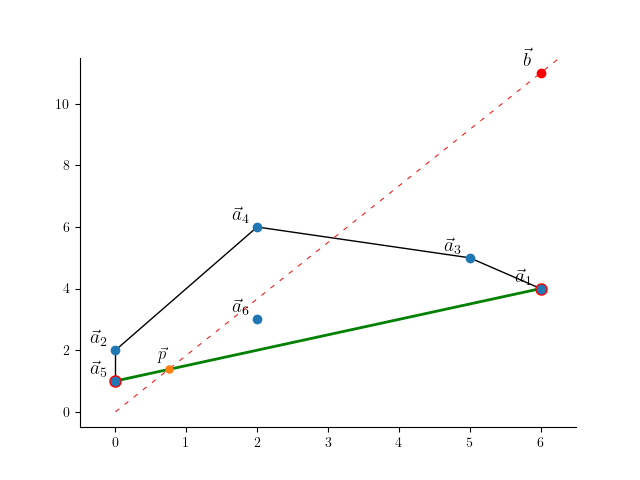
\includegraphics[width=0.5\columnwidth]{walkthrough_basis_selection.png}
    \caption{\label{fig:walkthrough_basis_selection} Basis selection }
\end{figure}
When you take a look at figure \ref{fig:walkthrough_basis_selection}, it is clear that the corners of the facet that got hit first by the ray to $\vec b$ are $\vec a_1 = (6, 4)^\top$ and $\vec a_5 = (0, 1)^\top$ and hence
$$A' := (\vec a_1, \vec a_5) = \mat{6&0\\4&1} \quad \Rightarrow \Delta(A') = \mat{6-0&4-1} = \mat{6&3}$$
Low let's perform the second step of the algorithm. It is easy to see that $\solspace(\Delta(A'), \vec 0) = \Span\smat{-1\\2}$ and because $\det A'^\top = 6 \neq 0$ we know that $\solspace(A'^\top, \vec 0) = \{\vec 0\}$ and we can thus choose $\vec\mu = \smat{-1\\2}$. (And also $\sprod{\vec\mu}{\vec a_1} = 2 > 0$)

Now we have to convert the $\vec\mu$ we found into the correct Gauß elimination steps $C$, so that $A' := C\cdot A$ is our optimized matrix. (Note: Here we are reusing the symbel $A'$ for a different purpose.) We do this according to lemma \ref{lemma:construct_gauss_steps}. We see that:
$$D := \mat{-1&0\\0&2} \quad\Rightarrow \tilde A = D \cdot A = \mat{-6&0&-5&-2&0&-2\\8&4&10&12&2&6}$$
To construct $C'$, we set $c := \max_{i\in[2], j\in[6]}|\tilde A_{ij}| = 12$ and thus:
$$C' = \imat_2 + \opmat_2(c) = \mat{13&12\\12&13} \quad\Rightarrow C = C'\cdot D = \mat{-13&24\\-12&26}$$
$$A' = C \cdot A = \mat{18&48&55&118&24&46\\32&52&70&132&26&54}\qquad \vec b' = C\cdot \vec b = \mat{186\\214}$$
This is our optimized $A$. With that we can now do again the construction from theorem \ref{theorem:column_sum_construction}. Let $s'_j$ be the $j$-th column sum of $A'$. $\alpha' = \max\{s'_1, \dots, s'_6\} = 118+132=250$, $v_j = \alpha - s_j$. Now let's define $k'$ and with that $\beta'$:

$$k' \geq \frac{1}{\min\{s'_1, \dots, s'_6\}} \sum_{i=1}^{2}b'_i = \frac{1}{24+26}(186+214) = 8 \quad \Rightarrow k' := 8$$ 
$$\beta' = k'\cdot\alpha' - \sum_{i=1}^{2}b'_i = 8\cdot250-(186+214) = 1600$$
This gives us the extended CCS ILP $(A'_{ext}, \vec b'_{ext}, \vec\omega'_{ext})$:
$$A'_{ext} = \mat{18&48&55&118&24&46&0\\32&52&70&132&26&54&0\\200&150&125&0&200&150&250}\quad\vec b':= \mat{186\\214\\1600}\quad \vec\omega'_{ext} = (1, 2, 3, 4, 5, 6, 0)^\top$$

By this method we brought the depth of the tree, in other wods the amount of layers, down from $k=17$ to $k'=8$, which will yield a way smaller graph. If we furthermore apply the graph optimisations discussed in chapter \ref{chap:graph_optimisation} and also remove childrenless vertecies, we can display the final graph in figure \ref{fig:walkthrough_final_graph}.
\begin{figure}
    \centering
    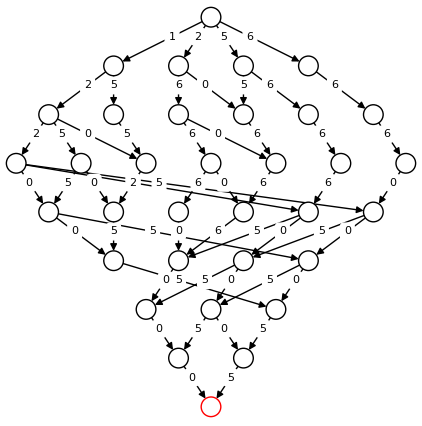
\includegraphics[width=0.5\columnwidth]{walkthrough_final_graph.png}
    \caption{\label{fig:walkthrough_final_graph} Graph constructed of $A'_{ext}$. Vertex values are hidden.}
\end{figure}

\subsection{Discussion on slack variables}
It is common that a ILP be given in its standard form. To be able to apply the proposed algorithm, you need to first convert it in slack form. As described in observation \ref{obs:lp_slack_form}, we will extend $A$ by an identity matrix.

This fact hugely impacts the results we can expect from the algorithm. Let's think it through: As all unit vectors are present as column vectors of $A$, they will impact the convex hull. More excactly, all these unit vectors lie on the hyperpla $x_1 + \dots + x_n = 1$ and as no point can be between the origin and this plane, this hyperplane will manifest itself as a facet of the convex hull. It is clear geometrically, that any ray cast from the origin to some point $\vec b$ will always hat this plane first. Consequently, this face will be selected by the algorithm which means, the selected basis will be the standart basis.

Hence $A'$ will be some column permutation of the identity matrix. You can easily check that $\Delta(A')\opvec(1) = \vec 0$ and $A'^T\opvec(1) = \opvec(1) \neq \vec0$. Thus the algorithm could pick $\vec\mu = \opvec(1)$.

Why is this an issues now? $\opvec(1)$ represents the matrix $A$ itself without alterations. And as the algorithm spits out the best possible matrix, we cannot imporve $A$ even further. 

Hence, any ILP given in its standard form is solveble within the shortest path framework but the execution can not be improved with the imporved method.
\chapter{Conclusion}
In this thesis, we revisited and extended the approach proposed by \cite{algebraic_statistics} for solving integer linear programming (ILP) instances by transforming them into instances of the shortest path problem on a directed and weighted graph. We focused on a broader class of ILP instances, allowing for varying column sums in the constraint matrix $A$.

Through my research, I have successfully extended the proposed algorithm to handle matrices with positive column sums, bringing a new perspective to ILP solving. Although our algorithm does not outperform existing approaches in terms of speed, it provides valuable insights and alternative strategies for solving ILP problems. The weakness in handling commonly used slack variables poses an additional problem for the applicability of the proposed algorithm.

The implications of our findings lie in the exploration of different viewpoints and techniques for ILP optimization. By extending the applicability of the algorithm to more general matrices, we open up possibilities for further research and development in this area.

Moving forward, further exploration into the extension of our approach to handle general whole number matrices. This could involve refining the algorithm and investigating additional strategies to improve its performance and efficiency.

Reflecting on the research process, I am grateful for the guidance and support provided by my advisor throughout this journey. Their encouragement allowed me to freely explore my mathematical intuition and pursue this research with passion.

% In closing, I would like to express my gratitude to all those who contributed to this thesis, and thank you for the opportunity to delve into this fascinating area of study.
% \chapter{Old stuff}
\section{Shortest Path Problems}
\subsection{Introduction}
% Something about the importance of this problem family
\subsection{All pairs shortest path}
Here we see the power of exchanging the semiring for the first time. In this section we will use the tropical semiring $(\R \cup \{\infty\}, \min, +)$ and its induced matrix operations. But first we have to state the problem:
\begin{problem}[All pairs shortest path] 
    Given a directed weighted graph $G = (V, E)$ with $|V| = n$ and $|E| = m$ and its adjacency matrix $A$. Compute the length of the shortest path between every pair of nodes.
\end{problem}

\begin{lemma}
    Let $A \in \R^{n \times n}$ be an adjacency matrix. Then $(A^k)_{ij}$ holds the length of the shortest path with $k+1$ nodes between $v_i$ and $v_j$ for all $k \in \N$. 
\end{lemma}
\begin{proof}
    Let $D_k \in \R^{n \times n}$ ba a matrix such that $(D_k)_{ij}$ holds the length of the shortest path with $k+1$ nodes between $v_i$ and $v_j$. Thus we need to show that $A^k = D_k$ for all $k \in \N$ which we will do by induction. Namely, we need to show that (I) $D_0 = \imat_n$ and (II) $D_{k+1} = D_k \odot A$
    \begin{enumerate}
        \item[(I)] ...
        \item[(II)] ...
    \end{enumerate}
\end{proof}

\begin{lemma}
    Let $A \in \R^{n \times n}$ be an adjacency matrix of a directed weighted graph $G$. Then $G$ has no negative cycle $\Leftrightarrow$ 
    $$\sum_{k=0}^{n-1+q} A^k = \sum_{k=0}^{n-1} A^k \quad\forall q \in \N$$
\end{lemma}

\begin{corollary}
    A direct conclusion of the last lemma is that
    $$A^* = \sum_{k=0}^{\infty}A^k = \sum_{k=0}^{n-1}A^k$$
\end{corollary}

And $A^*$ solves our problem.

\subsubsection{Optimisiation in shortest path}
As we allready stated, shortest path only exist iff no negative cycles are present in the graph. This also means that if loop edges exist, their weight must be positive. Thus no shortest path will pass through these loops, because any path passing through these edges can be shortened by just removing this edge. So even if loops exist in the graph, they can be ignored for the shortest path calculations. We will modify the graph such that every vertex has a loop with weight 0, resulting in a new adjacency matrix $\tilde A$:
$$\tilde A_{ij} = \begin{cases}
    0  &\textrm{if}\quad i = j\\
    A_{ij} &\textrm{else}
\end{cases}$$
And it will hold that
$$A^* = \sum_{k=0}^{n-1}\tilde A^k$$

Using the next lemma we can simplify our computation:
\begin{lemma}
    Let $(S, \oplus, \odot, 0, 1)$ be an semiring such that $\oplus$ is idempotent and $(S^{n \times n}, \boxplus, \boxdot, \zeromat, \imat)$ the semiring of matrix operations induced by $S$. Let $M, A \in S^{n \times n}$ such that $\forall i \in [n]: A_{ii} = 1$. Than it holds that:
    $$(M \boxdot A) \boxplus M = M \boxdot A$$ 
\end{lemma}
\begin{proof}
    \begin{align*}
        ((M\boxdot A) \boxplus M)_{ij} &= (M\boxdot A)_{ij} \oplus M_{ij} = (M\boxdot A)_{ij} \oplus( M_{ij} \odot \underbrace{A_{jj}}_1)\\
        &= (M_{i1} \odot A_{1j}) \oplus \dots \oplus (M_{ij} \odot A_{jj}) \oplus \dots \oplus (M_{in} \odot A_{nj}) \oplus (M_{ij} \odot A_{jj})\\
        &= (M_{i1} \odot A_{1j}) \oplus \dots \oplus (M_{in} \odot A_{nj}) \oplus \underbrace{(M_{ij} \odot A_{jj}) \oplus (M_{ij} \odot A_{jj})}_{(M_{ij} \odot A_{jj})}\\
        &= (M_{i1} \odot A_{1j}) \oplus \dots \oplus (M_{ij} \odot A_{jj}) \oplus \dots \oplus (M_{in} \odot A_{nj}) = (M \boxdot A)_{ij}
    \end{align*}
\end{proof}
Because $\tilde A$ has the neutral element of $\odot = +$ on its diagonal and $\oplus = \min$ is idempotent we can apply this lemma, resulting in $\tilde A^{k+1} \boxplus \tilde A^k = \tilde A^{k+1}$ and thus the sum for computing $A^*$ collapses to the simple expression:
$$A^* = \tilde A^{n-1}$$

This result could also be achieved by looking at the problem from the graph theory perspective. $A^*_{ij}$ holds the length of shortest path between $v_i$ and $v_j$ of any number of edges less than $n$. But if every vertex has a loop with weight 0, every such path can be extended to a path with $n-1$ edges while preserving its length. So every shortest path with less than $n-1$ edges is a shortest path with $n-1$ edges und thus $A^* = \tilde A^{n-1}$.
% Schnelle Matruxmult: https://www.sciencedirect.com/science/article/pii/S0020019008000719?fr=RR-2&ref=pdf_download&rr=7f1561f26f73aca3

\subsubsection{General Einsumisation of $A^*$}
To find a general expression in the language of Einsums we need to convert the sum of exponents in a sum of products. In this case we can actually boil it down to just one product. For this, we use this identity
$$\left(\begin{matrix}
    x & 1\\
    0 & 1
\end{matrix}\right)^k = \left(\begin{matrix}
    x^k & 1 + x + \dots + x^{k-1} \\
    0 & 1
\end{matrix}\right) \quad \forall k \in \N$$
which can be easily seen by induction. If we insert matrices instead of numbers in this two-by-two matrix and use the matrix operations induced by the semiring in use, we get
$$M(A) := \left(\begin{matrix}
    A & \imat\\
    \zeromat & \imat
\end{matrix}\right) \quad\Rightarrow\quad M(A)^n = \left(\begin{matrix}
    A^n & A^* \\
    \zeromat & \imat
\end{matrix}\right)$$
With this formulation, we can even drop the run-time form the previous $O(n^4)$ - $n$ matrix multiplications - to $O(n^3 \log n)$, because we can compute the $n$-th power of a matrix using $O(\log n)$ matrix multiplications. Using the Strassen-Algorithm for matrix multiplication we can even get down to $O(n^{\log_27}\log n)$.

The corresponding Einsum string is just the representation of matrix exponentiation:
$$it_1,t_1t_2,\dots, t_{n-2}t_{n-1},t_{n-1}j \rightarrow ij, M(A)$$

\subsubsection{Old derivation}
Our goal was more ambitious than just solving the problem. We wanted to state the solution in the language of Einsums. For that we need to go up one dimension. Let $R_{ijk} := A^{n-1}_{ij}$ be a tensor. Now we can rewrite $A^*$ as follows
$$A^*_{ij} = \sum_{k=0}^{n-1} A^k_{ij} = \sum_{k=1}^{n}A^{k-1}_{ij} = \sum_{k=1}^{n}R_{ijk}$$
This expression is allready in the necessary shape. The last step is to compute $R_{ijk}$. For that we need to define even more tensors: 
$$A^{(l)}_{ijk} := 
\begin{cases}
    A_{ij} & \textrm{if}\quad l \leq k\\
    \imat_{ij} & \textrm{else}   
\end{cases}
$$
As shown in Fig. \ref*{fig:shortest_path_tensor} we just need to multiply all matrices at each level together and than add the result up.

\begin{figure}[h]
    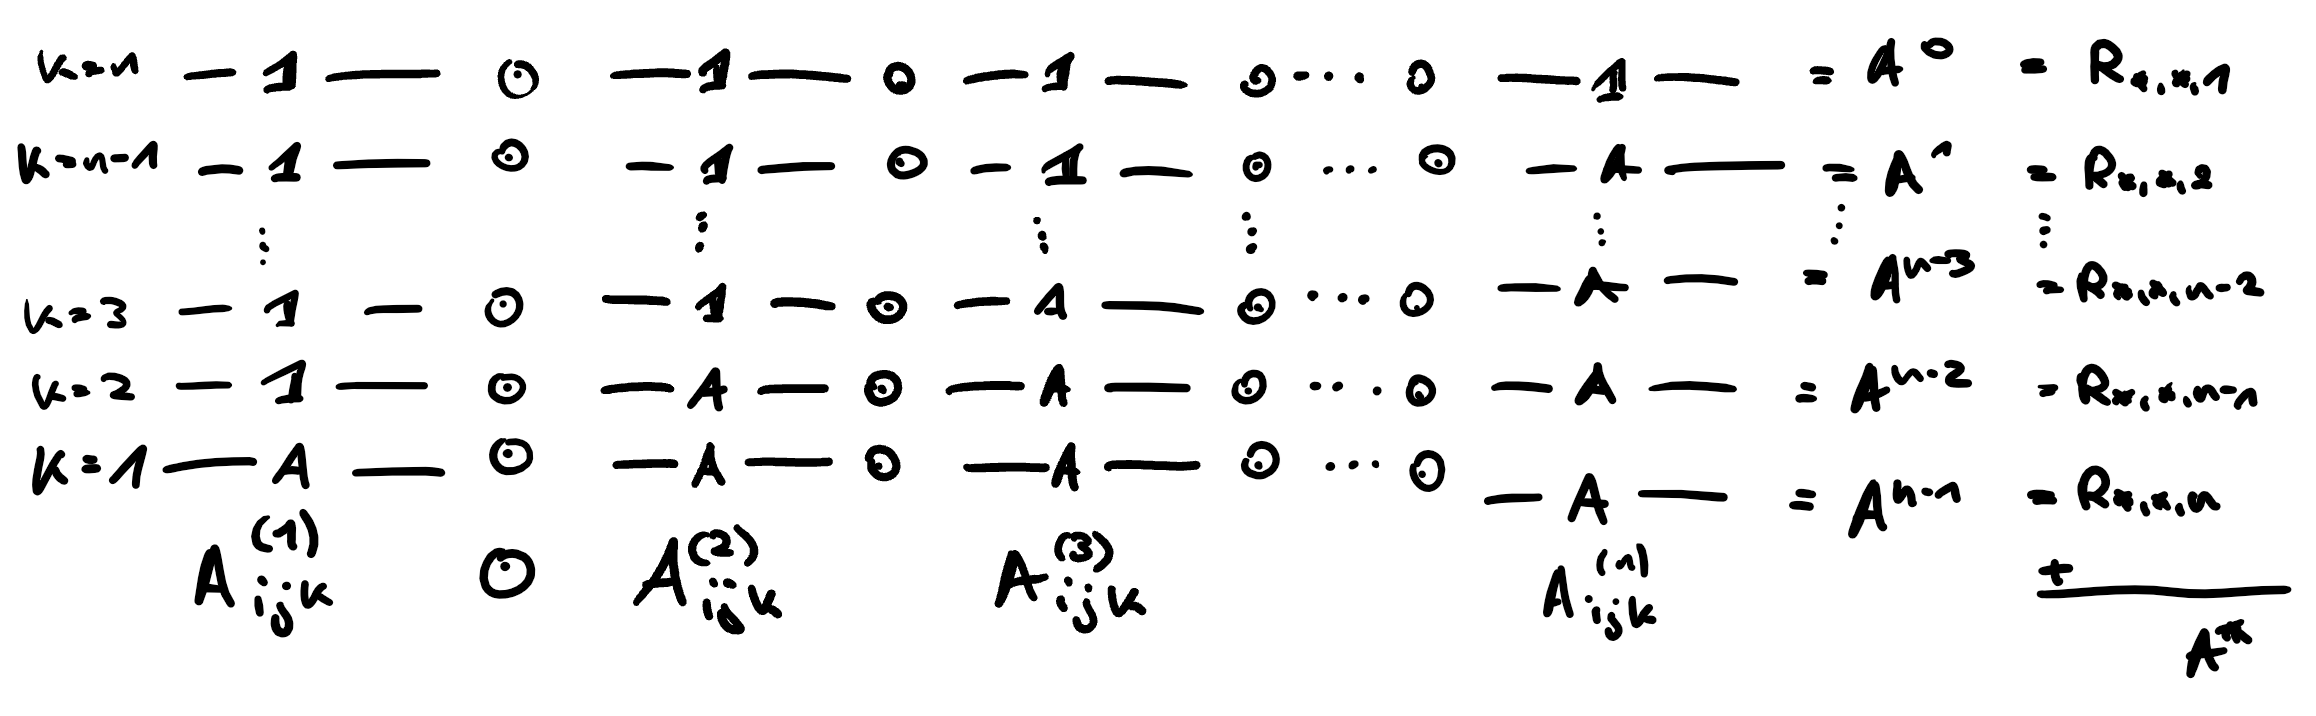
\includegraphics[width=\linewidth]{shortest_path_tensor.png}
    \caption{Visualized the shortest path tensors}
    \label{fig:shortest_path_tensor}
\end{figure}

The resulting expression comes out to be
$$A^*_{ij} = \sum_{k, t_1, \dots, t_{n-1} \in [n]} A^{(1)}_{it_1k}A^{(2)}_{t_1t_2k}A^{(3)}_{t_2t_3k}\dots A^{(n-1)}_{t_{n-2}t_{n-1}k}A^{(n)}_{t_{n-1}jk}$$
Which correspond to the Einsum string
$$it_1k, t_1t_2k, t_2t_3k, \cdots, t_{n-2}t_{n-1}k, t_{n-1}jk \to ij$$

\subsubsection{Receiving the paths}
To keep track of the paths we need to adapt the semiring. 
\begin{lemma}
    Let $V$ be a set then $(S := \R \times \powerset(\powerset(V)) \cup \{(\infty, \emptyset)\}, \oplus, \odot, (\infty, \emptyset), (0, \{\emptyset\}))$ is a semiring with the following operations:
    \begin{align*}
        (x_1, p_1) \oplus (x_2, p_2) &:= \begin{cases}
            (x_1, p_1) &\textrm{if}\quad x_1 < x_2 \\
            (x_2, p_2) &\textrm{if}\quad x_1 > x_2\\
            (x_1, p_1 \cup p_2) &\textrm{if}\quad x_1 = x_2
        \end{cases}\\
        (x_1, p_1) \odot (x_2, p_2) &:= (x_1 + x_2, \{s_1 \cup s_2 \mid s_1 \in p_1, s_2 \in p_2\}) =: (x_1 + x_2, p_1 \circ p_2)
    \end{align*}
\end{lemma}
\begin{proof}
    Because $\forall a \in \R\colon a < \infty$, $(\infty, 0)$ is indeed the neutral element of $\oplus$. The neutrality of $(0, \{\emptyset\})$ arises from the fact that $\forall (x, p) \in S\colon (x, p) \odot (0, \{\emptyset\}) = (x + 0, p \circ \{\emptyset\}) = (x, p)$. $(\infty, \emptyset)$ absorbs over $\odot$, because $\forall (x, p) \in S\colon (x, p) \odot (\infty, \emptyset) = (x + \infty, p \circ \emptyset) = (\infty, \emptyset)$. Commutivity and associativity of both $\oplus$ and $\odot$ result from the communativity and associativity of $+$, $\cup$ and $\circ$. If a $\infty$ is involved, these properties as well es distributivity also hold. Because $\odot$ is communative we only need to check left transitivity for when no $\infty$ is involved, namely 
    $$(x_1, p_1) \odot ((x_2, p_2) \oplus (x_3, p_3)) = ((x_1, p_1) \odot (x_2, p_2)) \oplus ((x_1, p_1) \odot (x_3, p_3))$$
    If $x_2 \neq x_3$ this is easy to see. Let w.l.o.g. $x_2 < x_3$ than we get
    \begin{align*}
        (x_1, p_1) \odot ((x_2, p_2) \oplus (x_3, p_3)) &= (x_1, p_1) \odot (x_2, p_2) = (x_1 + x_2, p_1 \circ p_2)\\
        ((x_1, p_1) \odot (x_2, p_2)) \oplus ((x_1, p_1) \odot (x_3, p_3)) &= (x_1 + x_2, p_1 \circ p_2) \oplus (x_1 + x_3, p_1 \circ p_3) = (x_1 + x_2, p_1 \circ p_2)
    \end{align*}
    Let us now consider the case $x_2 = x_3$.
    \begin{align*}
        (x_1, p_1) \odot ((x_2, p_2) \oplus (x_3, p_3)) &= (x_1, p_1) \odot (x_2, p_2 \cup p_3) = (x_1 + x_2, p_1 \circ (p_2 \cup p_3))\\
        ((x_1, p_1) \odot (x_2, p_2)) \oplus ((x_1, p_1) \odot (x_3, p_3)) &= (x_1 + x_2, p_1 \circ p_2) \oplus (x_1 + x_3, p_1 \circ p_3)\\ 
        &= (x_1 + x_2, (p_1 \circ p_2) \cup (p_1 \circ p_3))
    \end{align*}
    Thus, it is left to check whether $p_1 \circ (p_2 \cup p_3) \stackrel{?}{=} (p_1 \circ p_2) \cup (p_1 \circ p_3)$, in other words whether $\circ$ distributes over $\cup$.
    \begin{align*}
        x \in p_1 \circ (p_2 \cup p_3) &\Leftrightarrow \exists s_1 \in p_1, x' \in p_2 \cup p_3\colon x = s_1 \cup x'\\
        &\Leftrightarrow \exists s_1\in p_1, s_2 \in p_2, s_3 \in p_3 \colon x = s_1 \cup s_2 \cup s_3\\
        &\Leftrightarrow \exists s_1\in p_1, s_2 \in p_2, s_3 \in p_3 \colon x = (s_1 \cup s_2) \cup (s_1 \cup s_3)\\
        &\Leftrightarrow \exists x' \in p_1 \cup p_2, x'' \in p_1 \cup p_3 \colon x = x' \cup x''\\
        &\Leftrightarrow x \in (p_1 \circ p_2) \cup (p_1 \circ p_3)
    \end{align*}

    Closure is still to be checked and is not trivial, because all $(x, p)$ where $p \neq \emptyset$ are not in $S$. Let $(x_1, p_1), (x_2, p_2) \in S$. First assume $(x_1, p_1) \oplus (x_2, p_2) =: (x_3, p_3) \notin S$. The result must be in the form $x_3 = \infty, p_3 \neq \emptyset$. Thus, $x_1 = x_2 = \infty \Rightarrow p_1 = p_2 = \emptyset \Rightarrow p_3 = p_1 \cup p_2 = \emptyset$, which yields a contradiction.

    Let similarly assume $(x_1, p_1) \odot (x_2, p_2) =: (x_3, p_3) \notin S$. Again, it must hold that $x_3 = \infty, p_3 \neq \emptyset$. But $x_3 = \infty \Rightarrow x_1 = \infty \lor x_2 = \infty$. Let w.l.o.g $x_1 = \infty \Rightarrow p_1 = \emptyset$. $p_3 = p_1 \circ p_2 = \emptyset$, again a contraciction. Thus, $S$ is closed under $\oplus$ and $\odot$.
\end{proof}
Equipped with this semiring we can keep track of the paths. Let $V$ in the semiring be the set of edges. We build the adjacency matrix $A$ as follows:
$$A_{ij} = \begin{cases}
    (w(v_i, v_j), \{\{(v_i, v_j)\}\}) &\textrm{if}\quad i \neq j \land (v_i, v_j) \in V\\
    \infty &\textrm{if}\quad i \neq j \land (v_i, v_j) \notin V\\
    (0, \{\emptyset\}) &\textrm{if}\quad i = j
\end{cases}$$
Now $A^k_{ij}$ holds in the first component the weight of the shortest path between $v_i$ and $v_j$ with exactly $k$ edges and the second component holds all the paths. Here a path is represented by the set of its edges. As a shortest path will never pass an edge twice, this representation is sufficiant. 

\subsection{All pairs longest path}
The computation is exactly the same as in the All pairs shortest path problem. The only difference is the semiring in use. Here we need $(\R \cup \{-\infty\}, \max, +)$ and there must not exist a positive cycle. Then just compute $A^*$ and the entry $A^*_{ij}$ holds the longest path from $v_i$ to $v_j$. [Small note on convergency of $A^*$]

\subsection{Minimum weight spanning tree}
Here we need the observation that the edge $(v, u)$ is not included in the MST iff its weight is larger than the maximum weight of any path between $v$ and $u$. [Add proof] This we can model, by defining the weight of a path as the maximum of the weights of its edges. Then we compute the all pairs shortest path problem, but now we have exchanged the $+$-operation by the $\max$-operation, which means we have to use the $(\R \cup\{\infty\}, \min, \max)$ semiring. After computing $A^*$ we include the edge $(v_i, v_j)$ in the minimum weight spanning tree iff $A_{ij} \leq A^*_{ij}$.
[Diskuss conergency of $A^*$]

\subsection{Further Problems}
\begin{itemize}
    \item Marko Chaines. Using the semiring $([0, 1], +, \cdot)$ $A^k_{ij}$ holds the propability that an agent reaches $v_j$ starting at $v_i$ after $k$ steps if the weights of the edges symbolze the properbility that an agent moves along this edge.
    \item Reachability / Transitive hull. In an undirected unweighted graph, we ask the question whether a vertex $v_j$ is reachable starting at vertex $v_i$. For that we could just compute the shortest path and see whether $A^*_{ij}$ is infinite or not. But we can achieve the same with less information by just using the $(\{0, 1\}, \lor, \land)$ semiring and check whether $A^*_{ij} = 1$.
\end{itemize}


\section{Tropic polynomials}
Let $c_{e_1, \dots, e_m}(p)$ be the coefficiant in $p \in S[q_1, \dots q_m]$ of the monomial $p_1^{e_1}\dots p_m^{e_m}$. 

\begin{lemma}
    \label{lemma:prem_trop_poly}
    Let $A \in \N^{m \times n}$ and $w \in \R^n$. Let
    $$f := \bigoplus_{i=1}^{n} \sprod{w}{\hat e_i}\odot  q_1^{(A\hat e_i)_1}\dots q_m^{(A\hat e_i)_m} \in \T[q_1, \dots, q_m]$$
    be a tropic polynomial. Then it will hold that for all $l \in \N$
    $$c_{e_1, \dots, e_m}(f^{\odot l}) = \min\left\{\sprod{w}{v} \mid v \in \N^n, \sum_{i=0}^{n}v_i = l, Av=\smat{e_1\\\vdots\\e_m}\right\}$$
    Where $\min\emptyset:=\infty$.
\end{lemma}

\begin{proof}
    We will prove it by induction over $l$.
    \begin{itemize}
        \item[$l=0$:] $f^{\odot0} = 0$. There exists only one vector in $v \in \N^n$ such that $\sum_{i=0}^{n}v_i = 0$, which is the zero vector $\vec 0$. It is also clear that $\sprod{w}{\vec 0}= 0$ and $A\vec0=0$. So
        $$
            \min\left\{\sprod{w}{v} \mid v \in \N^n, \sum_{i=0}^{n}v_i = 0, Av=\smat{e_1\\\vdots\\e_m}\right\} = \begin{cases}
                0 &\textrm{if}\quad e_1, \dots, e_m = 0\\
                \infty &\textrm{else}
            \end{cases}
            \stackrel{\checkmark}{=}c_{e_1, \dots, e_m}(0)
        $$
        \item[$l=1$:] Because $\hat e_1, \dots, \hat e_n$ are all the vectors in $\N^n$, such that their components add up to 1, the equality is true by construction.
        \item[$l>1$:] Let $e := (e_1, \dots, e_m)^\top \in \N^m$
        \begin{align*}
            c_{e_1, \dots, e_m}(f^{\odot l}) &= c_{e_1, \dots, e_m}(f^{\odot (l-1)}\odot f) = \bigoplus_{\substack{f, g \in \N^m\\f+g=e}} c_{f_1, \dots, f_m}(f^{\odot (l-1)}) \odot c_{g_1, \dots, g_m}(f)\\
            &= \bigoplus_{\substack{f, g \in \N^m\\f+g=e}} \left(\bigoplus_{\substack{x \in \N^n\\\sum_{i=1}^{n}x_i = l-1\\Ax=f}}\sprod{w}{x}\right) \odot \left(\bigoplus_{\substack{y \in \N^n\\\sum_{i=1}^{n}y_i = 1\\Ay=g}}\sprod{w}{y}\right)\\
            &= \bigoplus_{\substack{f, g \in \N^m\\f+g=e}}\bigoplus_{\substack{x, y \in \N^n\\\sum_{i=1}^{n}x_i = l-1\\\sum_{i=1}^{n}y_i = 1\\Ax=f, Ay=g}} \underbrace{\sprod{w}{x} \odot \sprod{x}{y}}_{\sprod{w}{x+y} =: \sprod{x}{v}} = \bigoplus_{\substack{f, g \in \N^m\\f+g=e}}\bigoplus_{\substack{v \in \N^n\\\sum_{i=1}^{n}v = l\\Av=f+g=e}} \sprod{w}{v}\\
            &= \bigoplus_{\substack{v \in \N^n\\\sum_{i=1}^{n}v = l\\Av=e}} \sprod{w}{v} = \min\left\{\sprod{w}{v} \mid v \in \N^n, \sum_{i=0}^{n}v_i = l, Av=e\right\}
        \end{align*} 
    \end{itemize}
\end{proof}

\begin{theorem}
    Let $\min \stackrel{!}{=} w^\top x$ s.t. $Ax=b$ an ILP, such that all columns of $A$ sum up to the same number $\alpha \in \N^*$. We wat the ILP, to have solutions, so $k = \frac{1}{\alpha}\sum_{i=1}^{m}b_i \in \N$ exists. Let $f \in \T[q_1, \dots, q_m]$ be like in Lemma \ref{lemma:prem_trop_poly}, so 
    $$f := \bigoplus_{i=1}^{n} \sprod{w}{\hat e_i}\odot  q_1^{(A\hat e_i)_1}\dots q_m^{(A\hat e_i)_m}$$
    Then $c_{b_1, \dots, b_m}(f^{\odot k})$ solves the ILP 
\end{theorem}

\begin{proof}
    Because of Lemma \ref{lemma:ilp_pre1}, for all solutions $x \in \N^n$ of $Ax=b$ will hold that $\sum_{i=1}^{n}x_i = k$. No it is just a matter of rewriting the solution of the ILP and applying Lemma \ref{lemma:prem_trop_poly}.
    \begin{align*}
        \min\{\sprod{w}{x} \mid x \in \N^n, Ax=b\} &\stackrel{\ref{lemma:ilp_pre1}}{=} \min\left\{\sprod{w}{x} \mid x \in \N^n, \sum_{i=1}^{n}x_i = k , Ax=b\right\}\\
        &\stackrel{\ref{lemma:prem_trop_poly}}{=} c_{b_1, \dots, b_m}(f^{\odot k})
    \end{align*}
\end{proof}

\section{Old and wrong solution}
\subsection{Final writeup}
Now we need to find a $\vec\mu$ that minizes $k(\vec\mu)$. I will present the algorithm to find this $\vec\mu$ up front and then show that the result is actually correct. First we need to define an operation. 
\begin{definition}
    Let $M \in \N^{m\times n}$ be a matrix. Then $\Delta(M) \in \Z^{(n-1)\times m}$ is also a matrix such that 
    $$\Delta(M)_{i,j} = M_{j,i} - M_{j,i+1}$$
\end{definition}

\begin{algorithm}
    \label{_algo}
    \textbf{Input: } $A\in\N^{m\times n} \neq 0, \vec b \in \N^m$. Let $\vec a_1, \dots, a_n\in\N^m$ be the columns of $A$.\\
    \textbf{Output: } $\vec\mu\in\R^m$ that minimizes the function:
    $$k(\vec\mu) = \frac{\sprod{\vec\mu}{\vec b}}{\min_{j\in[n]}\sprod{\vec\mu}{\vec a_j}}$$
    Steps:
    \begin{enumerate}
        \item Sort all columns in $A$ by their column sum - $O(n \log n + m \cdot n)$
        \item Perform the choice of basis algorithm, to select a basis of the column space of $A$. Let the basis be $[\vec a_{j_1}, \dots, \vec a_{j_r}]$. Create a new matrix $A' := (\vec a_{j_1}, \dots, \vec a_{j_r}) \in \N^{m \times r}$ - $O(m^2 \cdot n)$
        \item Calculate $\Delta(A')$ and then a basis of $\solspace(\Delta(A'), \vec0)$ - $O(n^2 \cdot m)$
        \item Calculate a basis of $\solspace(A^\top, \vec0)$ - $O(n^2 \cdot m)$
        \item Find a $\vec\mu \in \solspace(\Delta(A'), \vec0) \setminus \solspace(A^\top, \vec0)$. For example write basis vectors of solution space of 4. on the left and basis vectors of solution space of 5. on the right in a matrix. Do basis selection. There will be a base vector selected from the right. This can be $\vec\mu$. - $O(m^3)$
    \end{enumerate}
    This yields a runtime of $O(n \cdot m^2 + n^2 \cdot m + m^3) = O(n^2 \cdot m + m^3)$.
\end{algorithm}

Now we have to answer the question of correctness. And we will do that in a few steps.
\begin{enumerate}
    \item Make sure, that the $\vec\mu$ actaully exists, meaning: $\solspace(\Delta(A'), \vec0) \setminus \solspace(A^\top, \vec0) \neq \emptyset$.
    \item Make sure, that the $\vec\mu$ is actaully in the domain of $k$, meaning $\vec\mu \in U \Leftrightarrow \forall j \in [n]\colon \sprod{\vec a_j}{\vec\mu}>0$.
    \item Make sure, that the $\mu$ minimizes $k(\vec\mu)$.
\end{enumerate}
First define some notions, that we will need throughout:
\begin{definition}
    \label{def:_algo_basic}
    Let $A \in \N^{m \times n}$ be a matrix, such that $A$ does not contain a zero column. Let $\vec a_j$ be the $j$-th column of $A$. Let $B := [\vec a_{j_1}, \dots, \vec a_{j_r}]$ and $A' \in \N^{m\times r}$ be as in step 2 in the algorithm \ref{algo}. Let $\vec b \in \N^m$. Let $U := \{\vec\mu \in \R^m\mid \forall j \in [n]\colon\sprod{\vec\mu}{\vec a_j} > 0\}$. Let $U_j := \{\vec\mu \in U \mid \forall j'\in[n]\colon \sprod{\vec\mu}{\vec a_j} \leq \sprod{\vec\mu}{\vec a_{j'}}\}$. Let $k\colon \N^m\to\R$ be defined as 
    $$k(\vec\mu) := \frac{\sprod{\vec\mu}{\vec b}}{\min_{j\in[n]}\sprod{\vec\mu}{\vec a_j}}$$
\end{definition}

\subsubsection{Existance of a result}
\begin{lemma}
    Let $A, A'$ be as in definition \ref{def:algo_basic}. Then $\dim(\solspace(\Delta(A'), \vec0)) > \dim(\solspace(A^\top, \vec0))$.
\end{lemma}
\begin{proof}
    Observe that $\dim(\solspace(\Delta(A'), \vec0)) = \nullity(\Delta(A'))$ and $\dim(\solspace(A, \vec0)) = \nullity(A)$. By construction: $\rank(A) = \rank(A^\top) = \rank(A') = r$. As $\Delta(A')$ has only $r-1$ rows, $\rank(\Delta(A')) \leq r-1 < r$. Now we can apply the Rank-nullity theorem to $A^\top$ and $\Delta(A')$.
    $$m = \rank(A^\top) + \nullity(A^\top) \Leftrightarrow \nullity(A^\top) = m - r$$
    $$m = \rank(\Delta(A')) + \nullity(\Delta(A')) < r + \nullity(\Delta(A'))\Leftrightarrow \nullity(\Delta(A')) > m - r$$
    Combining these two results yields $\nullity(\Delta(A')) > \nullity(A^\top)$ the result we wanted to show.
\end{proof}
The difference of 2 vector spaces, of which the first one has a bigger dimesnion, yields always a nonempty set of vectors. Thus indeed $\solspace(\Delta(A'), \vec0) \setminus \solspace(A^\top, \vec0) \neq \emptyset$. But not only that, it also ensures that the method of selecting a $\vec\mu \in \solspace(\Delta(A'), \vec0) \setminus \solspace(A^\top, \vec0)$ proposed in step 5 does yield a solution.

\subsubsection{Is the result of the algorithm a possible solution}
In this section we will show that $\vec\mu \in U \Leftrightarrow \forall j \in [n]\colon \sprod{\vec a_j}{\vec\mu}>0$. We know that by construction $\vec\mu \notin \solspace(A^\top, \vec0)$ which translates to $\forall j \in [n]\colon\sprod{\vec\mu}{\vec a_j} \neq 0$. Furthermore because $\vec\mu\in\solspace(\Delta(A'), \vec0)$ we know that $\sprod{a_{j'_1}}{\vec\mu} = \dots = \sprod{a_{j_r}}{\vec\mu} =: d$. We know that $d \neq 0$ and we can thus w.l.o.g. assume that $d>0$, because if $d$ would be negative, we could replace $\vec\mu$ by $-\vec\mu$ which would yield a positive $d$. It is left to show that the dot-product with all other columns of $A$ is also positive:

\begin{lemma}
    \label{lemma:non_basis_vecs_greater}
    Let $A$ and $[\vec a_{j_1}, \dots, \vec a_{j_r}]$ as in definition \ref{def:algo_basic}. Let $\vec a_l$ be any column of $A$, that did not get selected by the basis selection. Let $\vec\mu \in \R^m$ be a result from algorithm \ref{algo}, thus $\sprod{\vec a_{j_1}}{\vec\mu} = \dots = \sprod{\vec a_{j_r}}{\vec\mu} =: d > 0$. Then it will hold, that 
    $$\sprod{\vec a_l}{\vec\mu} \geq d$$
\end{lemma}
\begin{proof}
    As $\vec a_l$ was not selected as a basis, we know that it linearly dependend on the columns on its left in the matrix $A$, where the columns have been sorted by their column sum in an ascending order.  Let the set of basis vectors that are on the left of $\vec a_l$ be $\{\vec a_{j_1}, \dots, \vec a_{j_s}\}$. Thus we know that their column sum is never larger than the column sum of $\vec a_l$. In other words:
    $$\forall k \in [s]\colon\sum_{i=1}^{m} \left(\vec a_{j_k}\right)_i \leq \sum_{i=1}^{m} \left(\vec a_l\right)_i$$
    Because $\vec a_{j_l}$ is linearly dependend on those previous columns and the vectors $\vec a_{j_1}, \dots, \vec a_{j_s}$ are a basis of that space, we know that there must exist $\lambda_1, \dots, \lambda_s$ such that:
    $$\sum_{k=1}^{s}\lambda_k \vec a_{j_k} = \vec a_l$$
    Now we will consider the component sum of $\vec a_l$
    \begin{align*}
        \sum_{i=1}^{m} (\vec a_l)_i &= \sum_{i=1}^{m} \left(\sum_{k=1}^{s}\lambda_k \vec a_{j_k}\right)_i = \sum_{i=1}^{m} \sum_{k=1}^{s}\lambda_k \left(\vec a_{j_k}\right)_i = \sum_{k=1}^{s} \lambda_k \cdot\underbrace{\sum_{i=1}^{m} \left(\vec a_{j_k}\right)_i}_{\leq \sum_{i=1}^{m} (\vec a_l)_i}\\
        &\leq \sum_{k=1}^{s} \lambda_k \cdot\sum_{i=1}^{m} (\vec a_l)_i = \left(\sum_{k=1}^{s} \lambda_k\right) \cdot\left(\sum_{i=1}^{m} (\vec a_l)_i\right)\\
        \Rightarrow\quad 1 &\leq \sum_{k=1}^{s} \lambda_k
    \end{align*}
    With this result we are ready to compute the dot product.
    $$\sprod{\vec a_{l}}{\vec\mu} = \largesprod{\sum_{k=1}^{s}\lambda_k \vec a_{j_k}}{\vec\mu} = \sum_{k=1}^{s}\lambda_k \underbrace{\sprod{\vec a_{j_k}}{\vec\mu}}_d = d\cdot \underbrace{\sum_{k=1}^{s}\lambda_k}_{\geq 1} \geq d$$
\end{proof}
Now we know that for all columns of $A$, namely $\vec a_j$ it will hold that:
$$\sprod{\vec a_j}{\vec\mu} \geq d > 0$$

\subsubsection{Correctness of the solution}
Before we discuss whether we can indeed find the minimum, we determine what $k(\vec\mu)$ actually is, where $\vec\mu$ is the result of our algorithm. For that, we can still benefit from lemma \ref{lemma:non_basis_vecs_greater}. It says, that $\sprod{\vec a_{j_i}}{\vec\mu} = d$ is actually the smallest possible dot-product. Thus
$$k(\vec\mu) = \frac{1}{d}\cdot\sprod{\vec\mu}{\vec b}$$
Now we will see, that this is actually the smallest possible value. To see that remember that $k(\vec\mu)$ is piecewise strictly monotone or constant. It is apparent that the minimumn can only be reached in a montone region. Remember that (INSERT REF) $\restrict{k}{U_{j_1} \cap \dots \cap U_{j_r}}$ is constant iff $\vec b \in \Span(\vec a_{j_1}, \dots, a_{j_r})$. Thus we have to only consider all different basis of the column space in $A$. So if $[\vec a_{j'_1}, \dots, \vec a_{j'_r}]$ is a different basis from $[\vec a_{j_1}, \dots, \vec a_{j_r}]$, we need to show that $k(\vec\mu') \geq k(\vec\mu)$ for $\vec\mu \in U_{j_1} \cap \dots \cap U_{j_r}$ and $\vec\mu' \in U_{j'_1} \cap \dots \cap U_{j'_r}$. And this will be done by the next lemma:

\begin{lemma}
    Let $A$ and $B := [\vec a_{j_1}, \dots, \vec a_{j_r}]$ as in definition \ref{def:algo_basic} and let the columns of $A$ be sorted by their column sum in an ascending order. Let $B' := [\vec a_{j'_1}, \dots, \vec a_{j'_r}]$ be a different basis, also such that the vectors are sorted based on their column sum ascendingly. Let $\vec\mu \in U_{j_1} \cap \dots \cap U_{j_r}$ and $\vec\mu' \in U_{j'_1} \cap \dots \cap U_{j'_r}$, thus $\sprod{\vec a_{j_1}}{\vec\mu} = \dots = \sprod{\vec a_{j_r}}{\vec\mu} =: d > 0$ and $\sprod{\vec a_{j'_1}}{\vec\mu'} = \dots = \sprod{\vec a_{j'_r}}{\vec\mu'} =: d' > 0$. Then $k(\vec\mu) = k(\vec\mu')$.
\end{lemma}
\begin{proof}
    We will show that not only $\sprod{\vec a_{j'_1}}{\vec\mu'} = \dots = \sprod{\vec a_{j'_r}}{\vec\mu'} = d'$ but this also holds for $B$, namely $\sprod{\vec a_{j_1}}{\vec\mu'} = \dots = \sprod{\vec a_{j_r}}{\vec\mu'} = d'$. From this, is it clear that $\vec\mu' \in U_{j_1} \cap \dots U{j_r}$ and because $\restrict{k}{U_{j_1} \cap \dots U{j_r}}$ is constant and also $\vec\mu \in U_{j_1} \cap \dots U{j_r}$, we can conclude that $k(\vec\mu) = k(\vec\mu')$. So in the following we will show that indeed $\sprod{\vec a_{j_1}}{\vec\mu'} = \dots = \sprod{\vec a_{j_r}}{\vec\mu'} = d'$. This we will do in 3 steps:
    \begin{enumerate}
        \item The coordnates of any basis vector in $B'$ expressed in terms of $B$ sum up to 1.
        \item The coordnates of any basis vector in $B$ expressed in terms of $B'$ sum up to 1.
        \item Conclude that $\sprod{\vec a_{j_k}}{\vec\mu'} = d'$ for all $k \in [r]$
    \end{enumerate}

    Let $\vec a_{j'_l}$ be an arbitrary vector of $B'$. Obviously there exists a unique linear combination of the vectors $B$:
    $$\vec a_{j'_l} = \sum_{k=1}^{r}\lambda_k\vec a_{j_k}$$
    If $\vec a_{j'_l}$ is also in $B$, meaning that there exists a $s$ such that $\vec a_{j'_l} = \vec a_{j_s}$, that it will hold that $\lambda_s = 1$ and all other $\lambda_k$'s are zero. Thus
    $$\sum_{k=1}^{r}\lambda_k = 1$$

    Now we have to consider the case where $\vec a_{j'_l}$ is not part of $B$. As $\vec a_{j'_l}$ has not been selected in the choice of basis algorithm, it must be a linear combination of the basis vectors in $B$ that stand left in the sorted matrix $A$. Thus:
    $$\vec a_{j'_l} = \sum_{k=1}^{s}\lambda_k\vec a_{j_k} \qquad\textrm{with}\quad \forall k \leq s\colon\sum_{i=1}^{m}(\vec a_{j_k})_i \leq \sum_{i=1}^{m}(\vec a_{j'_l})_i$$
    This result yields us following when considering the column sum of $\vec a_{j'_l}$:
    \begin{align*}
        \sum_{i=1}^{m} (\vec a_{j'_l})_i &= \sum_{i=1}^{m} \left(\sum_{k=1}^{s}\lambda_k \vec a_{j_k}\right)_i = \sum_{i=1}^{m} \sum_{k=1}^{s}\lambda_k \left(\vec a_{j_k}\right)_i = \sum_{k=1}^{s} \lambda_k \cdot\underbrace{\sum_{i=1}^{m} \left(\vec a_{j_k}\right)_i}_{\leq \sum_{i=1}^{m} (\vec a_{j'_l})_i}\\
        &\leq \sum_{k=1}^{s} \lambda_k \cdot\sum_{i=1}^{m} (\vec a_{j'_l})_i = \left(\sum_{k=1}^{s} \lambda_k\right) \cdot\left(\sum_{i=1}^{m} (\vec a_{j'_l})_i\right)\\
        \Rightarrow\quad 1 &\leq \sum_{k=1}^{s} \lambda_k = \sum_{k=1}^{r} \lambda_k
    \end{align*}
    The last step - replacing $r$ with $s$ - just corresponds with the fact, that the linear combination of the basis vectors is unique. And as we have found one, that only include the first $s$ basis vectors, we know that $\lambda_{s+1} = \dots = \lambda_r = 0$

    Now remind yourself that, it must hold that $\vec\mu' \in U_{j'_1} \cap \dots \cap U_{j'_r}$ by assumption. This only happens, if $\sprod{\vec a_{j'_l}}{\vec\mu'} = d'$ gives the smallest dot-product. So all other dot-products are actually bigger. This we can also use:
    $$d' = \sprod{\vec a_{j'_l}}{\vec\mu'} = \sum_{k=1}^{s}\lambda_k\underbrace{\sprod{\vec a_{j_k}}{\vec\mu'}}_{\geq d'} \geq d'\cdot \sum_{k=1}^{s}\lambda_k \quad\Rightarrow 1 \geq \sum_{k=1}^{s}\lambda_k = \sum_{k=1}^{r}\lambda_k$$
    Combining these two results yields again
    $$\sum_{k=1}^{r}\lambda_k = 1$$
    This concludes the first step of our proof. Onto the second:

    The second step involves some change of basis. We have seen that the coordinates of the basis vectors in $B'$ based on $B$ add up to 1. Let $T$ be the change of basis matrix from $B'$ to $B$. The abovementioned property can be reframed, as that the column sum of every colum in $T$ is equal to 1. Or in other words that $\opvec(1)^\top T = \opvec(1)^\top$. This property also holds for its inverse, because of this:
    $$\opvec(1)^\top T = \opvec(1)^\top \Leftrightarrow \opvec(1)^\top T\cdot T^{-1} = \opvec(1)^\top\cdot T^{-1} \Leftrightarrow \opvec(1)^\top = \opvec(1)^\top\cdot T^{-1}$$
    Thus if you express a basis vector from $B$ in coordinates of $B'$, the component sums ends up to be 1 as well. Let $\vec a_{j_l}$ be an arbitrary vector from the first basis. We thus know that
    $$\vec a_{j_l} = \sum_{k=1}^{r}\lambda'_k \vec a_{j'_k} \qquad \textrm{with}\quad \sum_{k=1}^{r}\lambda'_k = 1$$
    This concludes the second step in the proof. The last step is very short:
    $$\sprod{\vec a_{j_l}}{\vec\mu'} = \largesprod{\sum_{k=1}^{r}\lambda'_k \vec a_{j'_k}}{\vec\mu'} = \sum_{k=1}^{r} \lambda'_k \underbrace{\sprod{\vec a_{j'_k}}{\vec\mu'}}_{=d'} = d' \cdot \underbrace{\sum_{k=1}^{r} \lambda'_k}_{=1} = d'$$
\end{proof}

\subsection{Discussion on slack variables}
Normally, an ILP is not given as a system of equations $A\vec x = \vec b$, where all entries in $\vec x$ are natural numbers, but a system of inequalities $A\vec x \leq \vec b$, where all entries in $\vec x$ are whole numbers. This notation does not make immediate sense, as it seams like we are comparing two vectors with a $\leq$-sign. What is ment is, that for each component of $A\vec x$ must be smaller or equal the the corresponding component in $\vec b$. 

To convert from the the $\leq$-version to the $=$-version, you introduce another variable vector $\vec s$, resulting in linear system of equations:
$$A\vec x + \vec s = \vec b \qquad \vec x \in \N^n, \vec s \in\N^m$$
The variables in $\vec s$ are called slack variables. But instead of changing the equation we are dealing with, we can also just modify $A$ and $\vec x$ to get to the same result. If you just attach the vector $\vec s$ onto $\vec x$: $\vec x \mapsto (x_1, \dots, x_n, s_1, \dots, s_m)^\top \in \N^{n+m}$ and attach an identity matrix into $A$: $A \mapsto (A \mid\imat_m) \in \N^{m \times (n + m)}$. Thus, if we construct $A$ using the common method of slack variables, the columns of $A$ will include all possible unit vectors.

This fact hugely impacts the results we can expect from the algorithm. Let us think it through: When sorting the columns of $A$ by their column sum, all of these columns will be sorted to the beginning, as they have the minimal column sum of $1$. Because we have all standart basis vectors in the front of $A$, they will all be selected by the choice of basis algorithm. Thus $A'$ will be some column permutation of the identity matrix. You can easily check that $\Delta(A')\opvec(1) = \vec 0$ and because all column sum in $A$ are postive, this means that $A^\top \opvec(1) > \vec 0$. Thus the algorithm could pick $\vec\mu = \opvec(1)$.

Why is this an issues now? $\opvec(1)$ represents the matrix $A$ itself without alterations. And as the algorithm spits out the best possible matrizes, we cannot imporve $A$ even further. Which means, that of we use slack variables, the resulting matrix is not improvable.
\bibliography{thesis}
\addcontentsline{toc}{chapter}{Bibliography}
\newpage
\thispagestyle{empty}
\section*{Eigenständigkeitserklärung}
\begin{enumerate}
  \item Hiermit versichere ich, dass ich die vorliegende Arbeit selbstständig verfasst und keine
  anderen als die angegebenen Quellen und Hilfsmittel benutzt habe.
  Ich trage die Verantwortung für die Qualität des Textes sowie die Auswahl aller Inhalte und habe sichergestellt, dass Informationen und Argumente mit geeigneten wissenschaftlichen Quellen belegt bzw. gestützt werden. Die aus fremden oder auch eigenen, älteren Quellen wörtlich oder sinngemäß übernommenen Textstellen, Gedankengänge, Konzepte, Grafiken etc. in meinen Ausführungen habe ich als solche eindeutig gekennzeichnet und mit vollständigen Verweisen auf die jeweilige Quelle versehen. Alle weiteren Inhalte dieser Arbeit ohne entsprechende Verweise
  stammen im urheberrechtlichen Sinn von mir.
  \item Ich weiß, dass meine Eigenständigkeitserklärung sich auch auf nicht zitierfähige, generierende KI-
  Anwendungen (nachfolgend "generierende KI") bezieht.
  Mir ist bewusst, dass die Verwendung von generierender KI unzulässig ist, sofern nicht deren
  Nutzung von der prüfenden Person ausdrücklich freigegeben wurde (Freigabeerklärung). Sofern
  eine Zulassung als Hilfsmittel erfolgt ist, versichere ich, dass ich mich generierender KI lediglich als
  Hilfsmittel bedient habe und in der vorliegenden Arbeit mein gestalterischer Einfluss deutlich
  überwiegt. Ich verantworte die Übernahme der von mir verwendeten maschinell generierten
  Passagen in meiner Arbeit vollumfänglich selbst.
  Für den Fall der Freigabe der Verwendung von generierender KI für die Erstellung der vorliegenden
  Arbeit wird eine Verwendung in einem gesonderten Anhang meiner Arbeit kenntlich gemacht.
  Dieser Anhang enthält eine Angabe oder eine detaillierte Dokumentation über die Verwendung
  generierender KI gemäß den Vorgaben in der Freigabeerklärung der prüfenden Person.
  Die Details zum Gebrauch generierender KI bei der Erstellung der vorliegenden Arbeit inklusive Art,
  Ziel und Umfang der Verwendung sowie die Art der Nachweispflicht habe ich der Freigabeerklärung
  der prüfenden Person entnommen.
  \item Ich versichere des Weiteren, dass die vorliegende Arbeit bisher weder im In- noch im Ausland in
  gleicher oder ähnlicher Form einer anderen Prüfungsbehörde vorgelegt wurde oder in deutscher
  oder einer anderen Sprache als Veröffentlichung erschienen ist.
  \item Mir ist bekannt, dass ein Verstoß gegen die vorbenannten Punkte prüfungsrechtliche
  Konsequenzen haben und insbesondere dazu führen kann, dass meine Prüfungsleistung als
  Täuschung und damit als mit "nicht bestanden" bewertet werden kann. Bei mehrfachem oder
  schwerwiegendem Täuschungsversuch kann ich befristet oder sogar dauerhaft von der Erbringung
  weiterer Prüfungsleistungen in meinem Studiengang ausgeschlossen werden.
\end{enumerate}
\vspace{1cm}
Jena, den 07.\ März 2024
\vspace{0.5cm}\\
\includegraphics[width=0.2\textwidth]{Unterschrift.png}\\
Moritz Seppelt

\end{document}